\documentclass[12pt]{article}

\usepackage{sbc-template}
\usepackage{graphicx,url}
\usepackage[round, numbers]{natbib}


%\usepackage[brazil]{babel}   
\usepackage[utf8]{inputenc}  

     
\sloppy

\title{Gamified Language Learning: Enhancing Learning through Streaming Services and SRS}

\author{J. Emanuel Cascone R. S.\inst{1}, Guilherme A. Avelino\inst{1} }


\address{Computer Science Department - Federal University of Piauí (UFPI)\\
  Teresina, PI -- Brazil
  \email{\{emanuelcascone,gaa\}@ufpi.com.br}
}  
\begin{document} 

\maketitle

\begin{abstract} 
  The ability to learn a new language is directly related to the user's disposition and comfort for better interaction with learning platforms. This facilitates the gamification of language learning, thereby reducing its level of exhaustion. The process of learning a new language typically commences with activities such as writing, reading, listening, and speaking. This work involved creating an application that facilitates language learning by utilizing a movie streaming platform with subtitles, allowing users to watch movies with the original audio and subtitles and focus on keywords or frequently repeated words for better comprehension. The work is based on the premise that to understand a text, you don't necessarily need to know the whole formation but rather just the keywords or most repeated words, allowing you to apply skimming and scanning techniques. To record these words in the user's memory, gamified forms of Spaced Repetition System (SRS) can be applied to induce the user to better adapt to each scenario in the future based on their current repertoire. By following this approach, users can enhance their experience while watching movies or videos to acquire knowledge of a new language. \\
  \textbf{Key words:} language learning, gamification, streaming platforms, subtitles, SRS, skimming, scanning
\end{abstract} 


\section{Introduction}
Mastering a new language is undeniably valuable, yet it's often accompanied by challenges such as waning motivation and a sense of discomfort. What if there was a way to transform language acquisition into an engaging and less taxing experience? Imagine users effortlessly learning while enjoying themselves. \\
In parallel, watching movies and series has become a widespread and enjoyable activity, with streaming platforms emerging as a popular source of entertainment. This trend is evident from the data depicted in Figure-\ref{fig:netflix_quarter} and Figure-\ref{fig:disney_quarter}, illustrating the growth of Disney+ and Netflix over the years. Currently, there are over 700 million users across all platforms (Forbes home, 2022).Many individuals utilize these platforms to enhance their language skills by utilizing subtitles and audio for learning purposes. 
\begin{frame}{}
  \begin{figure}[h]
      \begin{minipage}[b]{0.45\linewidth}
          \centering
          \caption{Netflix subscribes from 2011 until 2023. font: company data}
          \label{fig:netflix_quarter}
          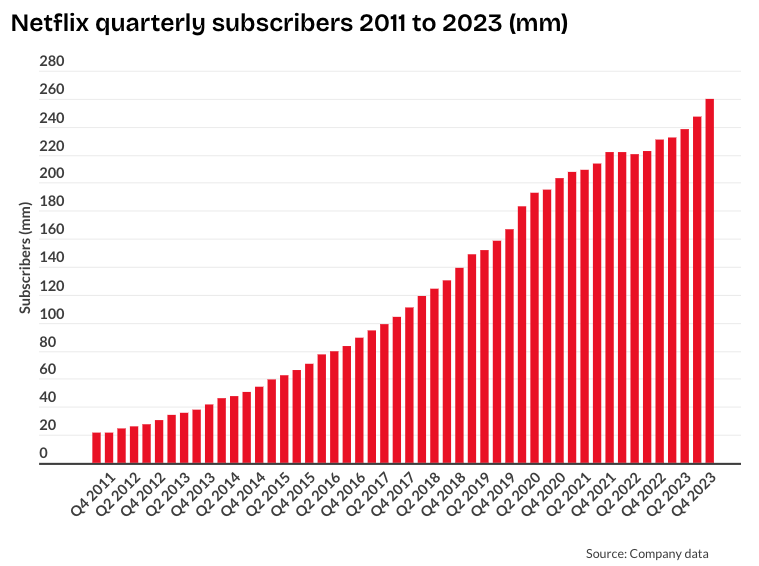
\includegraphics[width=1\textwidth]{assets/27.png}
          \label{fig:netflix_quarter}
      \end{minipage}
      \hspace{0.2cm}
      \begin{minipage}[b]{0.55\linewidth}
          \centering
          \caption{Disney subscribes from 2011 until 2023. font: company data}
          \label{fig:disney_quarter}
          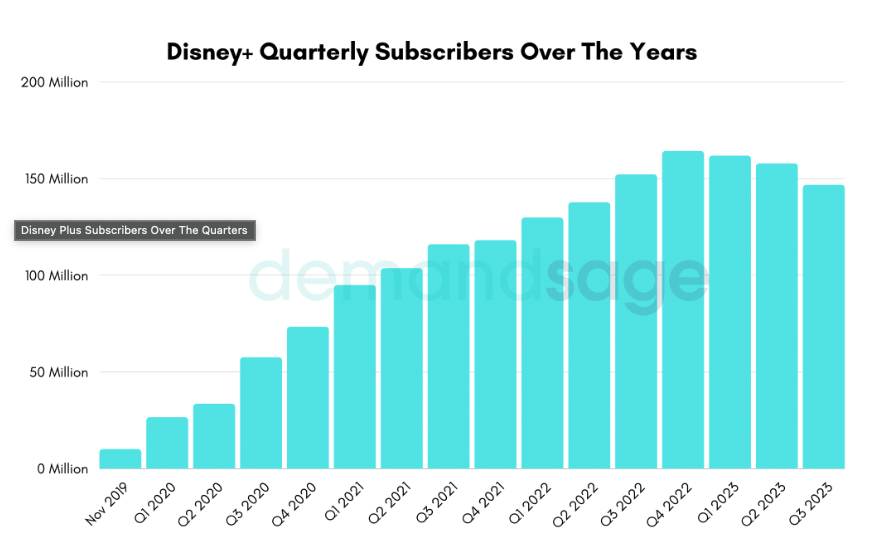
\includegraphics[width=1\textwidth]{assets/28.png}
          \label{fig:b}
      \end{minipage}
  \end{figure}
\end{frame}
Studies demonstrate that students acquire a new language at double the speed using a similar learning mechanism called smart subtitles \cite{Kovacs13}. Thus, it is feasible to infer that approaches involving entertainment platforms can also be practical for learning, especially when utilizing subtitles from these platforms.
The fusion of these concepts has the potential to help language learning, making it more engaging and less taxing. This work is about the creation of an application that allows users to learn a new language or expand their vocabulary in a gamified and interactive manner using streaming platforms.

\subsection{Motivation}
 Create new alternatives to make learning a new language more exciting and efficient is the motivation for this work. Because the conventional language learning method can be tiresome and demotivating for many students. \\
By creating an environment that allows interaction with streaming sites for movies, learning a new language can be done more naturally and playfully, similar to tools that translate web pages to facilitate learning or understanding of other languages already present in the market or research area \cite{ElBatanony21}. \\
By watching movies with audio and subtitles in the original language, the user can learn while applying gamified Spaced Repetition System (SRS) techniques to memorize new words. In succinct terms, the motivation for this work is to provide an efficient and attractive alternative for learning new languages.

\subsection{Problem Statement}
The traditional method of learning a new language can be exhausting and demotivating for many students. A more playful and interactive approach to learning new languages is necessary to make the process more enjoyable and efficient. 
To illustrate this, we notice that the current learning method creates a massive flow of giving up; an empirical example is "only 55, or 19\% of 286 Year 11 students reported that they intended to continue studying the language after age 16. The four most frequently cited reasons for not continuing were (a) that they did not enjoy it (35 students), (b) it was difficult (25 students), (c) it was of no use for their planned career (23 students), and (d) they were not good at it (20 students)" \cite{Graham1}. 

\subsection{General goals}

This work aims to develop an application that allows users to learn a new language or expand their vocabulary in a gamified and interactive manner. The extension will be designed to interact with movie streaming sites, leveraging the available subtitles on these sites to aid in the teaching process. \\
The work is based on the premise that learning a new language more efficiently and satisfactorily is possible when gamified and interactive. Additionally, it is based on a similar methodology - smart subtitles - which has been effective in expanding vocabulary \cite{Kovacs14}. \\
Thus, the goal is to offer a different and efficient approach to using subtitles so that people can learn new languages and expand their vocabulary while watching their favorite movies in a relaxed and effective way.



\section{Methodology}
To achieve the work's objectives, in this article we followed a methodology based on the following steps:
The first step was a literature review and gathering references for similar works or theoretical foundations to turn language learning into a more playful and interactive experience. \\
The second step was the study of methods for user training to improve the user's progress and how to manage the user information, including their progression in learning to make the learning process more efficient. \\
The third step was to build a prototype based on the previous steps, to test the idea and the user experience. \\
\subsection{First Step}

The literature review identified \cite{ElBatanony21} and \cite{Kovacs14} regarding subtitles in movies and their role in language learning. However, it is evident from apps like Flex and others that utilize this methodology that users do not receive training tailored to their individual word difficulty levels.  \\
Apps such as Duolingo, Memrise, Busuu, Lingoda, and Drops employ algorithms that adapt to the specific difficulties of each user. While the exact algorithms are not disclosed, users can observe word repetition in different contexts during the training process. This technique, known as Spaced Repetition System (SRS), facilitates user study. Moreover, gamification is integral to these apps, enhancing language learning and potentially improving both user experience and the learning process. \\
Current methods utilizing subtitles often result in recurrent breaks, as users must pause the movie to view translations by clicking on words or may need to read dual subtitles simultaneously. Another technique involves translating only the difficult parts of a phrase (smart subtitles), but this lacks interactivity and playfulness. 
\subsection{Second Step}

The second step focused on understanding the functionalities of language learning apps like Duolingo and others, and how to enhance both user experience and the learning process. \\
In 2024, it is notable that these apps leverage gamification to make learning less taxing. Games form the core of the learning process, compelling users to engage actively. For instance, Duolingo incorporates skimming and scanning techniques, presenting phrases and words in various contexts either to teach new words or to facilitate understanding without requiring knowledge of every word. \\ 

\subsection{Third Step}

This step aimed to integrate the four identified cores: SRS, gamification, scanning, and skimming, with the addition of "smart" functionality to subtitles. Users should be trained based on their individual difficulties, without interrupting the enjoyment of watching a video or movie with constant breaks for word translations. \\ 
The proposed solution involves creating an application that teaches users before watching the movie, eliminating the need for interruptions. This application should be interactive and playful, incorporating games to enhance both user experience and learning outcomes while employing SRS techniques.\\ 
\subsubsection{Approach to Goal Attainment}
The extension, site, and app development process involves distinct steps to achieve the overarching goal. While some steps are common across all environments, each has its unique set of tasks to accomplish the goal. \\
The development of the extension was based on the following requisites:  
\begin{enumerate}
  \item Capture subtitles from streaming sites.
  \item Send the subtitles to the database.
  \item Create a extension, site, and app to interact with the user.
  \item Create a modal with the iframe to show the site.
  \item Create a web channel to communicate with the site.
  \item Create a database to store the user information.

\end{enumerate}

\section{Theoretical Referential}
In recent years, there has been a growing interest in the use of subtitled videos as a way to assist in the learning of foreign languages. However, standard subtitles are not ideal for vocabulary acquisition, as translations are non-literal and are provided only for phrases, not individual words. \\
To overcome this problem, "Smart Subtitles" have been developed, interactive subtitles focused on vocabulary acquisition. "Smart Subtitles" includes features such as vocabulary definitions when hovering over with the mouse cursor and video navigation based on dialogue \cite{Kovacs13}. Studies have shown that students learn more than double the vocabulary with "Smart Subtitles" compared to Chinese-English dual subtitles, with similar levels of comprehension and satisfaction \cite{Kovacs14}. \\ he learning of foreign languages is the use of browser extensions. The browser extension "InteractiveSubtitle" \cite{ElBatanony21} is an example of this. The extension features personalized learning, translation of phrases in context on web pages, and support for over 100 languages. The goal is to utilize various hypotheses of foreign language acquisition to create a new language learning tool that is more effective. \\ 
Some students of languages don't adopt this method but adopt methods such as SRS, which is a technique tested and proved effective by Landauer and Bjork in 1978, that involves reviewing information at increasing intervals. This technique is used in apps like Anki, Duolingo, and others, and is a technique that is used to improve the user experience and learning outcomes. \\
Based on these ideas, an application has been proposed that utilizes a real kind of "Smart Subtitles" to train users through gamified practice before watching a subtitled movie in a language they are learning.   \\
Also, to improve the user commodity, an app and a site were proposed to not necessarily use a computer to study, providing a way for the user to study on every device. 
\subsection{Subtitles}
Smart subtitles and dual subtitles have emerged as innovative solutions to enhance the multilingual viewing experience for audiences worldwide. These technologies leverage advancements in natural language processing and multimedia to provide seamless translation and accessibility options for viewers. \\
Dual subtitles offer a unique viewing experience by presenting multiple languages simultaneously on-screen. This method is particularly beneficial for language learners and bilingual audiences seeking to improve their language proficiency. The concept of dual subtitles has been explored by scholars such as Dr. François Yvon, who has investigated its effectiveness in language acquisition and comprehension.\\
Smart subtitle technologies are integrated into streaming platforms and media players, allowing users to enable translation features with a simple toggle. Companies like Fleex and Language Reactor have invested in smart subtitle solutions to cater to their diverse global audience. The implementation of dual subtitles often involves specialized software tools or custom video players capable of displaying multiple subtitle tracks simultaneously. \\
Studies conducted by researchers such as Dr. Spela Vintar and Dr. Koen van Turnhout have demonstrated the effectiveness of smart subtitles and dual subtitles in improving language learning outcomes and comprehension rates. Their research highlights the potential of these technologies to bridge language barriers and promote cross-cultural understanding in multimedia contexts.\\
Smart subtitles and dual subtitles represent significant advancements in the field of multimedia translation and accessibility. By leveraging cutting-edge technologies and insights from scholars like Alex Waibel, François Yvon, Spela Vintar, and Koen van Turnhout, these methods offer new possibilities for enhancing the multilingual viewing experience and promoting linguistic diversity in digital media.
\subsection{Spaced Repetition System (SRS)}
Spaced Repetition Systems (SRS) have revolutionized the way we learn and retain information. The concept of spaced repetition dates back to the 19th century, but it gained significant attention and refinement in the digital era. This method leverages the psychological spacing effect, where information is better retained when revisited at increasing intervals over time. \\
One of the most influential implementations of SRS is \textit{SuperMemo}, developed by Dr. Piotr Wozniak in the late 1980s. SuperMemo was one of the first computer-based systems designed to optimize the learning process through spaced repetition algorithms. Wozniak's work has inspired numerous SRS applications and research studies worldwide.\\
Research conducted by cognitive psychologists such as Dr. Sebastian Leitner further validates the effectiveness of spaced repetition. Leitner introduced the \textit{Leitner system}, a practical implementation of spaced repetition using flashcards arranged in different boxes based on recall success. His work demonstrates how SRS can enhance long-term retention compared to traditional learning methods.\\
Spaced Repetition Systems offer a promising approach to optimize learning and memory retention. From pioneers like Hermann Ebbinghaus to modern innovators like Piotr Wozniak and Sebastian Leitner, the study of SRS continues to evolve, shaping the future of education and cognitive science.


\section{Software Design}
The application core (the method of teaching) is based on the articles by Kovács et al. \cite{Kovacs14}, which use the premise of subtitles to advocate for a more playful and immersive learning method. This demonstrates the potential of such approaches for language learning and how more playful and intelligent approaches directly influence learning new words, as exemplified in Figure-\ref{fig:my_label}. 
\begin{figure}[!h]
\centering
\caption{Learning curves for new words using two types of subtitles and smart subtitles}
\label{fig:my_label}
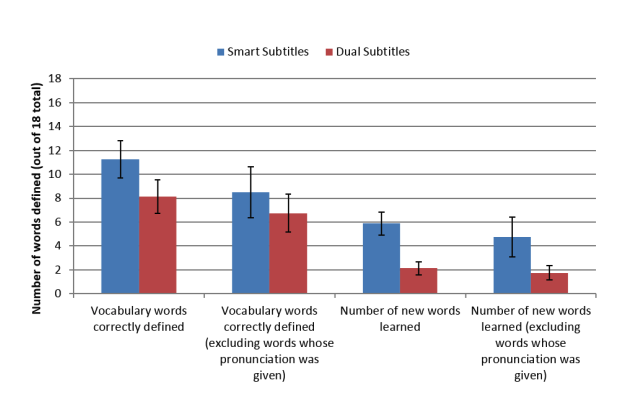
\includegraphics[width=0.7\textwidth]{assets/3.png}
\end{figure} 
\begin{figure}[!h]
  \centering
  \caption{
    Container Diagram for the application
  }
  \label{fig:container_diagram}
  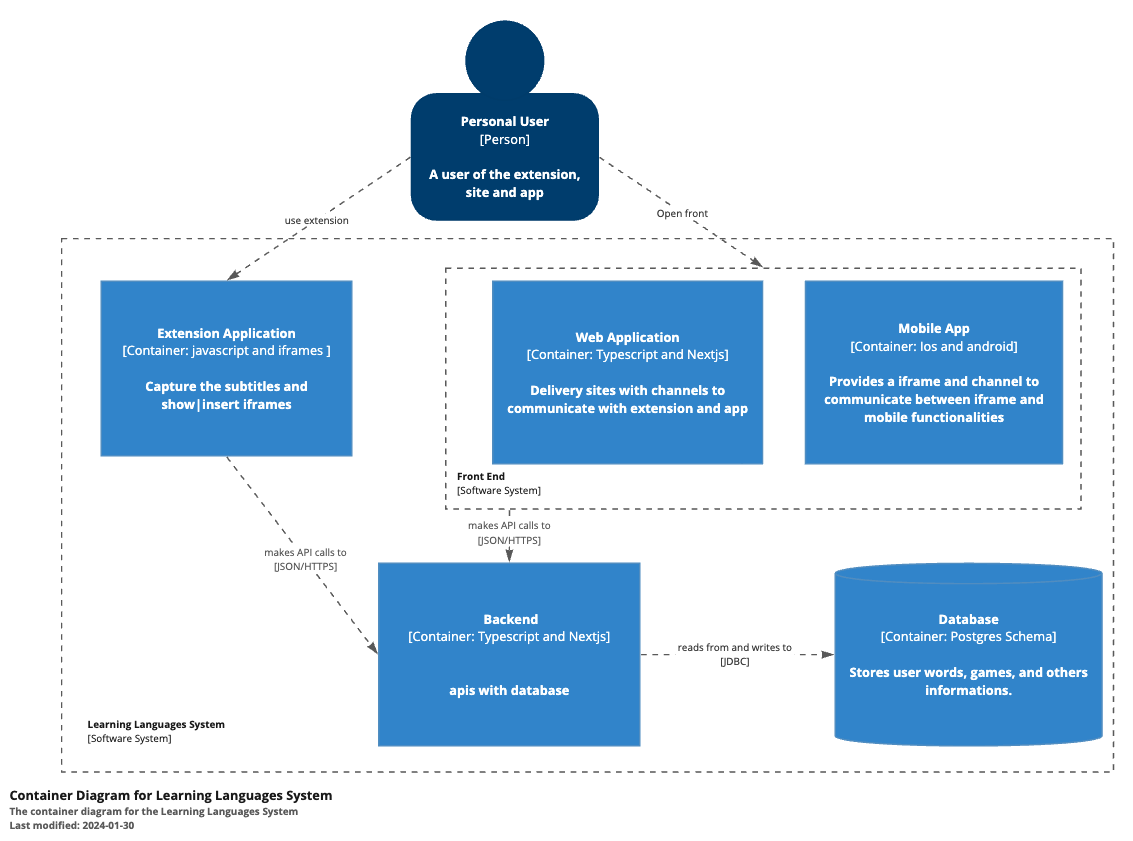
\includegraphics[width=0.9\textwidth]{assets/24.png}
\end{figure}

\begin{figure}[!h]
  \centering
  \caption{
    The flow of the application until the use of AI
  }
  \label{fig:flow_diagram}
  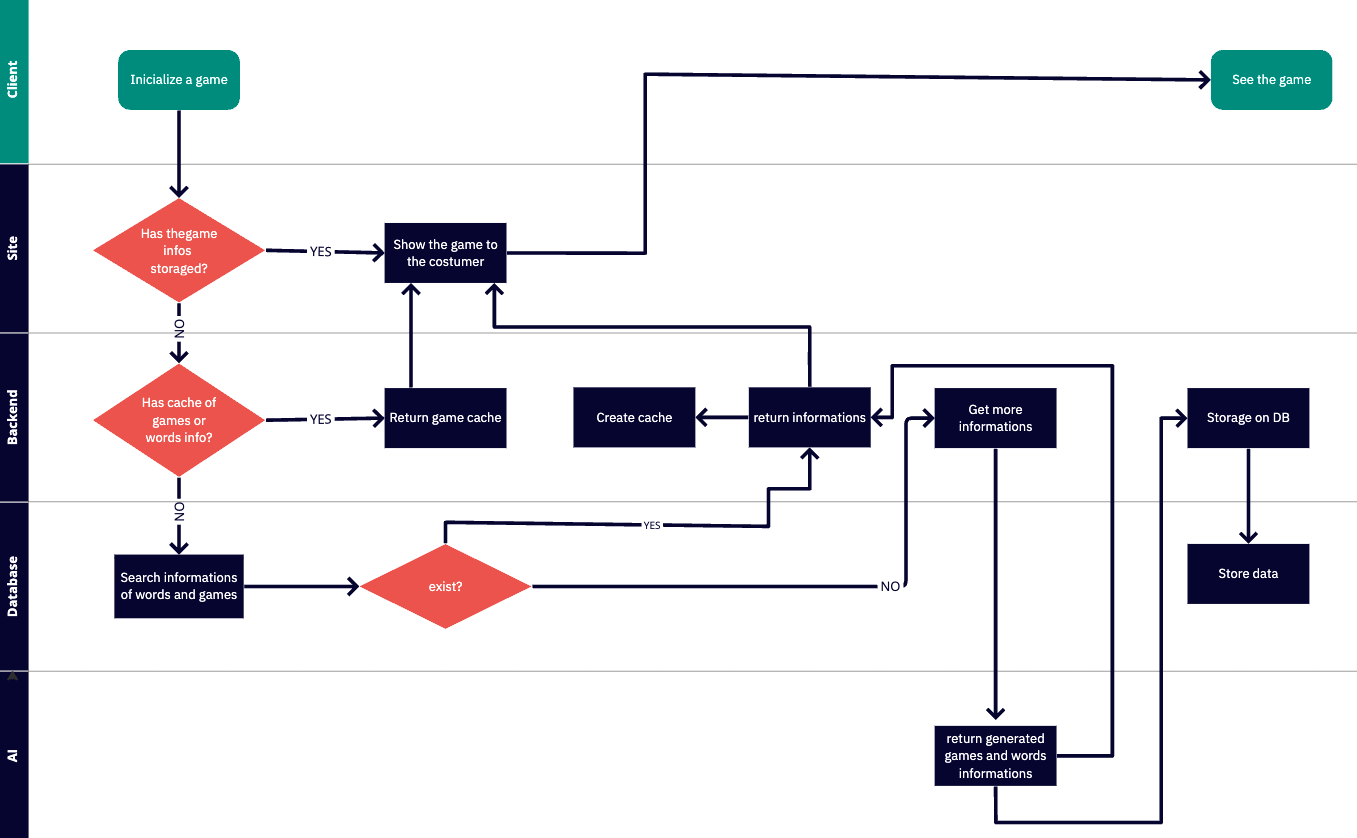
\includegraphics[width=0.9\textwidth]{assets/26.png}
\end{figure}
The work utilizes techniques used by El Batanony et al. in their article "A browser extension to facilitate language acquisition" \cite{ElBatanony21}, making the beginning of the development a case study of their article, observing the approach they used to create an extension that interacts with web pages.  \\
Using Spaced Repetition System (SRS) techniques to gamify learning new languages based on the premise that knowledge of keywords or the most repeated ones allows for text comprehension. \\
Created using modern technologies, including JavaScript, Typescript, HTML, CSS, Prisma, Nextjs, PostgreSQL, and Web Channels. This work also utilizes the browser's internal messaging services to integrate the extension with streaming sites. The extension works with Prime Video, but the goal is to expand to other platforms like Netflix, Disney+, and others. \\
The technologies were chosen based on the need to create a fast and efficient application with a good user experience and an excellent database to store user information and progression. Nextjs is a frontend and backend that has a big community and is very fast, having a good integration with Prisma, an ORM (Object-Relational Mapping) that is easy to use and has a good amount of users with PostgreSQL database. \\
Another important point to consider when using PostgreSQL is the existence of sites like Heroku, which provides a free database with a good amount of data and a good speed, and the existence of a good amount of users and documentation. \\
At this point in the prototype creation, an environment to learn a new language was built, including a browser extension, a site, and an app, all integrated and working together to provide a better experience. \\
The Container diagram, depicted in Figure-\ref{fig:container_diagram}, offers a detailed visualization of the application's architecture, delineating the interactions between different components such as the extension, site, and app. This diagram showcases the technological framework utilized and elucidates how these components collaborate to facilitate seamless communication and functionality. \\
The core of the system is an AI provided by openAI, to generate translations, meanings, and games. Each one of the environments has its own functions and responsibilities. The extension is responsible for capturing the subtitles and opening the modal with the iframe, the site is responsible for storing the data and providing the games, and the app is responsible for showing the site inside the iframe and sending the user information to the site. \\
To be more visible the process of the games and word data acquisition, the figure-\ref{fig:flow_diagram} illustrates it. This flow was selected with a focus on optimizing speed due to the substantial volume of data involved, along with the associated costs of utilizing AI. \\
Presently, the AI of choice is the gpt-3.5-turbo-0125 model developed by OpenAI, incurring costs of   input is \$0.50/1M tokens (the unit used in AI system) and output is  \$1.50 / 1M tokens. Leveraging a database for storing data offers greater flexibility, particularly since the input remains constant. This approach ensures that when a user learns a word in a specific language and transitions to another, the necessary information about games and the word parameter are retrieved from the AI only once. 
\subsection{Extract algorithm}
The filter algorithm is a critical component of the application, as it is responsible for identifying and extracting words from subtitles. For each platform (e.g., Prime Video, Netflix, Disney+), the algorithm must be tailored to the specific structure of the subtitles. \\
The algorithm is inserted into the extension and is responsible for capturing the subtitles and sending them to the site. \\
But the result is the same for all platforms, a JSON structure with the following content:

\begin{verbatim}
{
  words: {    
    word: string;
    count: number;
    moments: {
      begin: string;
      end: string;
      text: string;
    }[];
    position: number;
    percentage: number;
    total: number;
  },
}
\end{verbatim}
The algorithm run a pipiline that take the subtitle in TTML format and convert to JSON format, and then process the JSON to extract the words and their respective counts, phrases where the word exists, and determine the position and percentage of each word. \\
The algorithm is designed to asynchrony, without damaging the user experience, as it must process a large volume of data. The algorithm is also designed to be flexible, as it must be tailored to the specific structure of the subtitles for each platform. 
\subsection{AI}
  The AI is a critical component of the application, as it is responsible for providing translations, meanings, and games. The AI receives a prompt based on the user's request, and the AI returns the requested information. 
  An example of the prompt is: \\
  \begin{verbatim}
    I am a bot that generates quizzes for you to learn 
    new words. 
    My quiz is not very good at it, but I am learning.
    Help me to learn by generating a quiz.
    The quiz is a phrase using a word in the language and you 
    need to translate to the target language.
    The options are a list of words to choose the correct 
    translation for the word in the target language. 
    And the options are made by others translations on the 
    target language or translation of similar words.
    ```
    ...rest of the prompt contend an 
    example of input and output expected by the AI
    ```
  \end{verbatim}
  Currently, the prompt is used to generate the quiz, but AI is employed also to generate translations and meanings of the words. Once the AI receives the prompt and returns the requested information, the backend processes and stores it in the database. Storing the quiz is crucial because each request to the AI incurs a cost, which is determined by the number of tokens used in the request. \\
  If the approach were to manually create a database and quizzes, both the cost and time investment would significantly increase, leading to a deterioration in user experience. Given the large number of words required to generate a quiz, users would face a substantial learning curve in acquiring a new language.

\subsection{The games}
  The games are developed to transform the learning process singleton, which means that each word has its own line of learning and when appears on the user screen the user does something that answers if the user knows the word or not. \\
  Choose three games to generate, the first one is a quiz, the second one is a word search, and the third one is a flashcard. \\
  The quiz shows a phrase using a word in the language and the user needs to choose a correct translation for the word in the target language. The options are made by the AI. \\
  The word search is about showing a word in the language and the user needs to find the correct translation for the word in the target language. The options are made by the AI. \\
  The flashcard goal is  a word in the language and the user needs to choose whether he knows the word or not. \\
  Those games are designed based on apps like Anki and Duolingo.
\subsection{Learning algorithm}
Based on SRS and the games generated by the information provided by the AI, as the games are designed to transform the learning process singleton when the API sends information about the word, the game will show based on priority specificated on the API. \\
More priority is that the word will appear on the user screen, and the user will see the word more often. \\
The server(API) creates a ranking of words and the priority of the word to appear on the user screen. The api sorts and filters the words based on three parameters: 
\begin{enumerate}
  \item Is today the day for learning?
  \item How often does it repeat? 
  \item Are there any errors?
\end{enumerate}
Following exactly those questions the server(API) creates a ranking and filters the words. 
\subsubsection{Is today the day for learning?}
As the API uses an SRS technique, the API needs to know if today is the day for learning the word. The approach chosen was an exponential function, that is based on the number of times that the user saw the word and when the user made a mistake. The function is based on the following formula:
\begin{equation}
  \label{eq:1}
  f(x, y) = 2^x 
\end{equation}
Is a simple equation, for example: if the user sees the word today and doesn't make a mistake, he will see the word again in 2 days, if the user continues without making a mistake, he will see the word again in 4 days, and so on. But if the user makes a mistake, the function will be reset and the user will see the word again in 1 day. \\
That question filters the words that the user will see today. 
\subsubsection{How often does it repeat?}
The server also knows how common is this word (based on the entire database) and how common this word is on subtitles. The server gets the percentage of the word in the subtitle and the percentage of the word in the entire database, and based on that sort creates a ranking of the words. \\
Each of that information is 50\% of that ranking, and the server creates a ranking based on that information. 
\subsubsection{Are there any errors?}
The API also knows how many errors the user makes with that word, and how many errors the entire database makes with that word. The API gets the percentage of the word in the subtitle and the percentage of the word in the entire database, and based on that the server creates a ranking of the words. \\
As in the previous step, the server creates a ranking based on that information, taking 50\% of the database and 50\% of the user. \\




\section{Results}
A browser extension was developed that interacts with movie streaming sites and extracts the subtitles available on these sites. The extension uses Spaced Repetition System (SRS) techniques to gamify learning new languages based on the premise that knowledge of keywords or the most repeated ones allows for text comprehension. The goal is to expand to other platforms like Netflix, Disney+, and others. \\ 
The site was also developed to provide statistics on user progress, including the most challenging words, the total words learned, and others to help the user understand their learning process. The site also supports multiple languages, which allows users to learn a wide range of languages using AI translations and the creation of games.  \\
The app was developed to provide a way for the user to study on every device, displaying the iframe with the application site.\\
This work has demonstrated the potential of using technology to facilitate language learning. Integrating our tool with everyday activities such as watching movies can make language learning more engaging and compelling. 
\subsection{Interface}
As a result, each environment has its functions and responsibilities, and based on that it needs a different interface(resources) to have a better responsibility and user experience. And improve the features that each environment possible. The user can interact with the application with the ambient mobile and browser, using the app, site, or extension. Each interface is different and has different layouts and features to improve the user experience. 
\subsubsection{site}
The module of the site has an interface that adjusts to the user's device. The site is the base of the extension and app, and those use an iframe to show the site. The design is based on long and small screens to support the user in every device. The site also provides a way to communicate with the extension and the app, and the user can access the site to continue training the words from the streaming platform. Some examples of ways to interact with the application are:
\begin{itemize}
\item   Languages Page: where the user started to learn, the possible movies to study, and the movies that the user has started, as demonstrated in the figure-\ref{fig:site1}.
\item Language List: A List of languages that the user can learn, as demonstrated in the figure-\ref{fig:site2} and in the mobile version in the figure-\ref{fig:app2};
\item Profile Page: The user profile with progress for each language, as demonstrated in the figure-\ref{fig:site3}.
\item Languages by Movie: A list of languages when the user selects a movie, as demonstrated in the figure-\ref{fig:site4}.
% \item Example of game, as demonstrated in the figure-\ref{fig:site6}.
% \item Example of the Memory game, as demonstrated in the figure-\ref{fig:site7}.
% \item Example of the Quiz game, as demonstrated in the figure-\ref{fig:site8}.
\end{itemize}

\begin{frame}{}
  \begin{figure}[!h]
      \begin{minipage}[b]{0.5\linewidth}
        \centering
        \caption{
        Initial site interface for the user with the languages, movies, and started movies.
         }
        \label{fig:site1}
        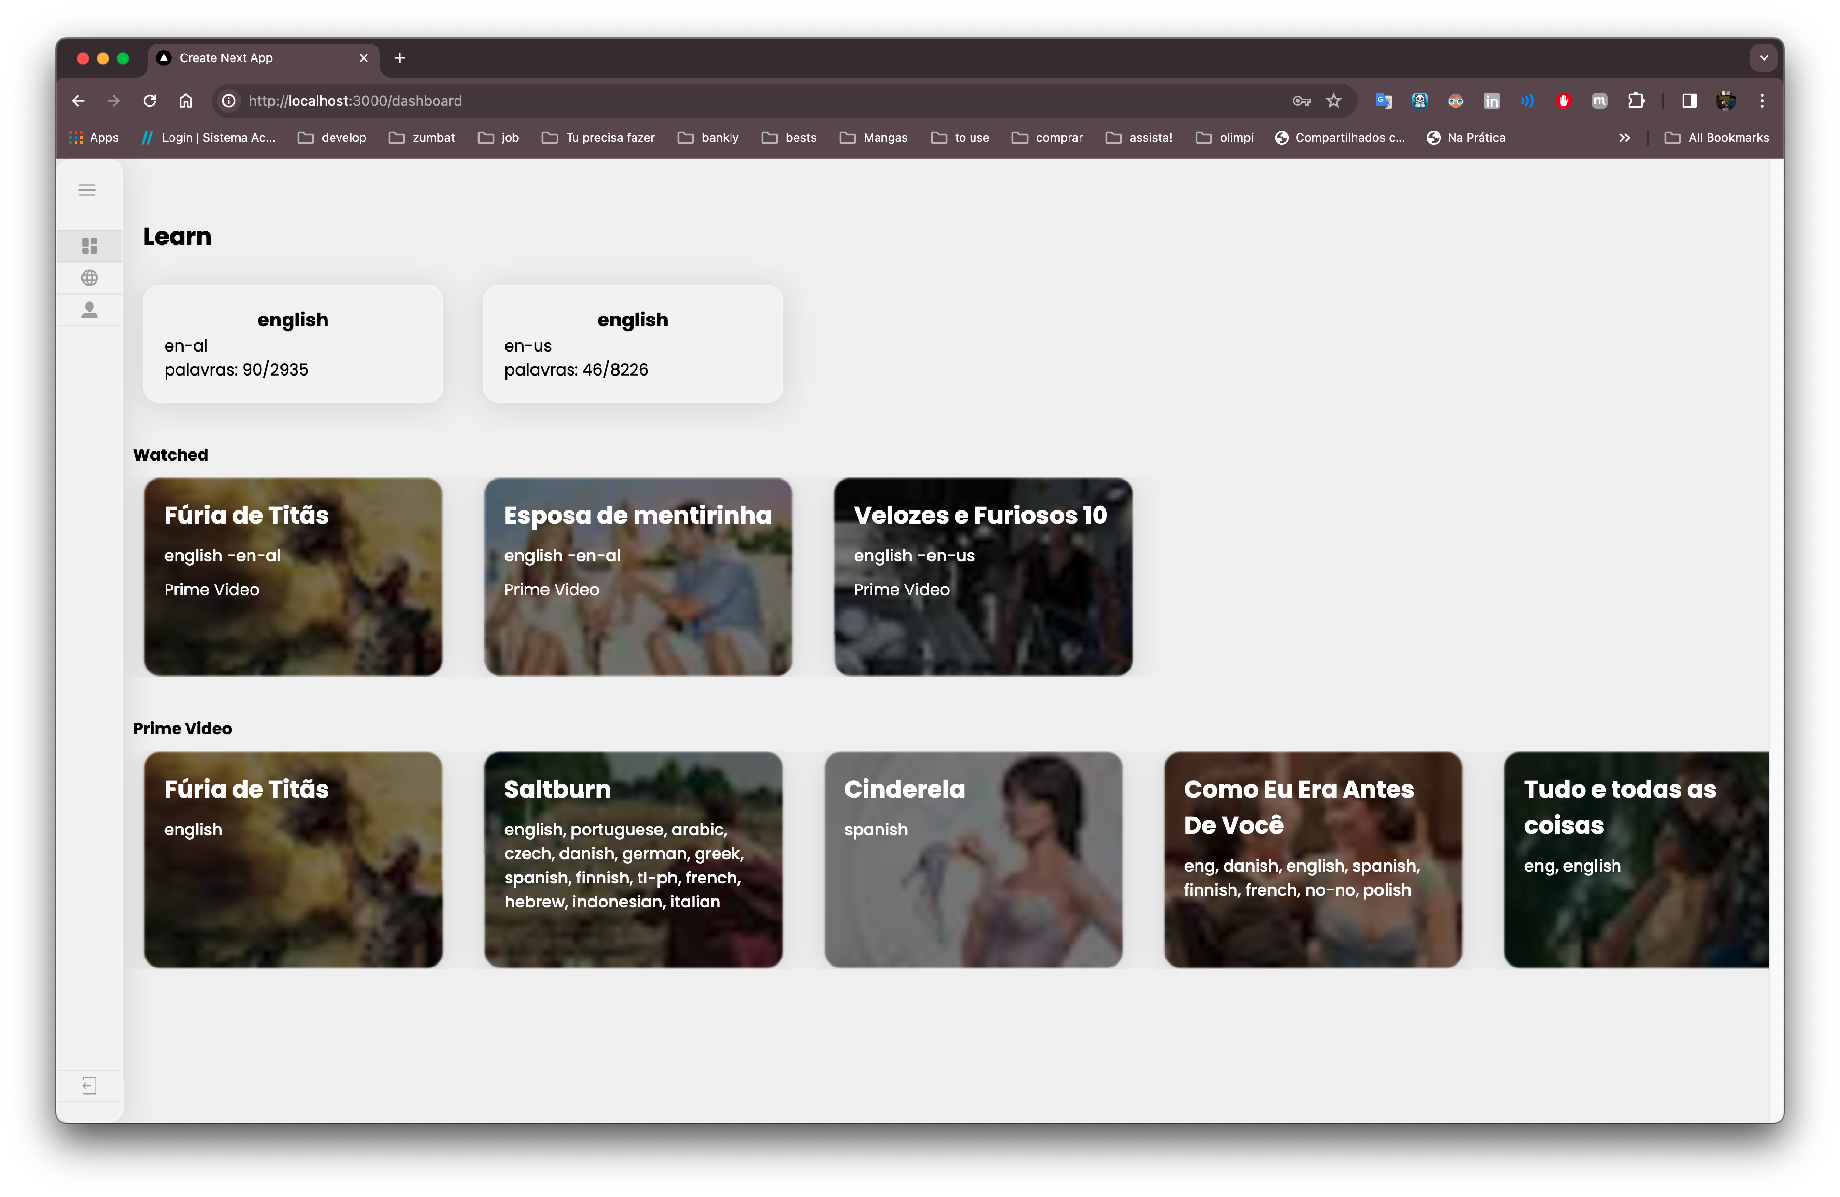
\includegraphics[width=1\textwidth]{assets/20.png}

      \end{minipage}
      \hspace{0.2cm}
      \begin{minipage}[b]{0.5\linewidth}
        \centering
        \caption{
        A list of languages that the user can learn. 
        }
        \label{fig:site2}
        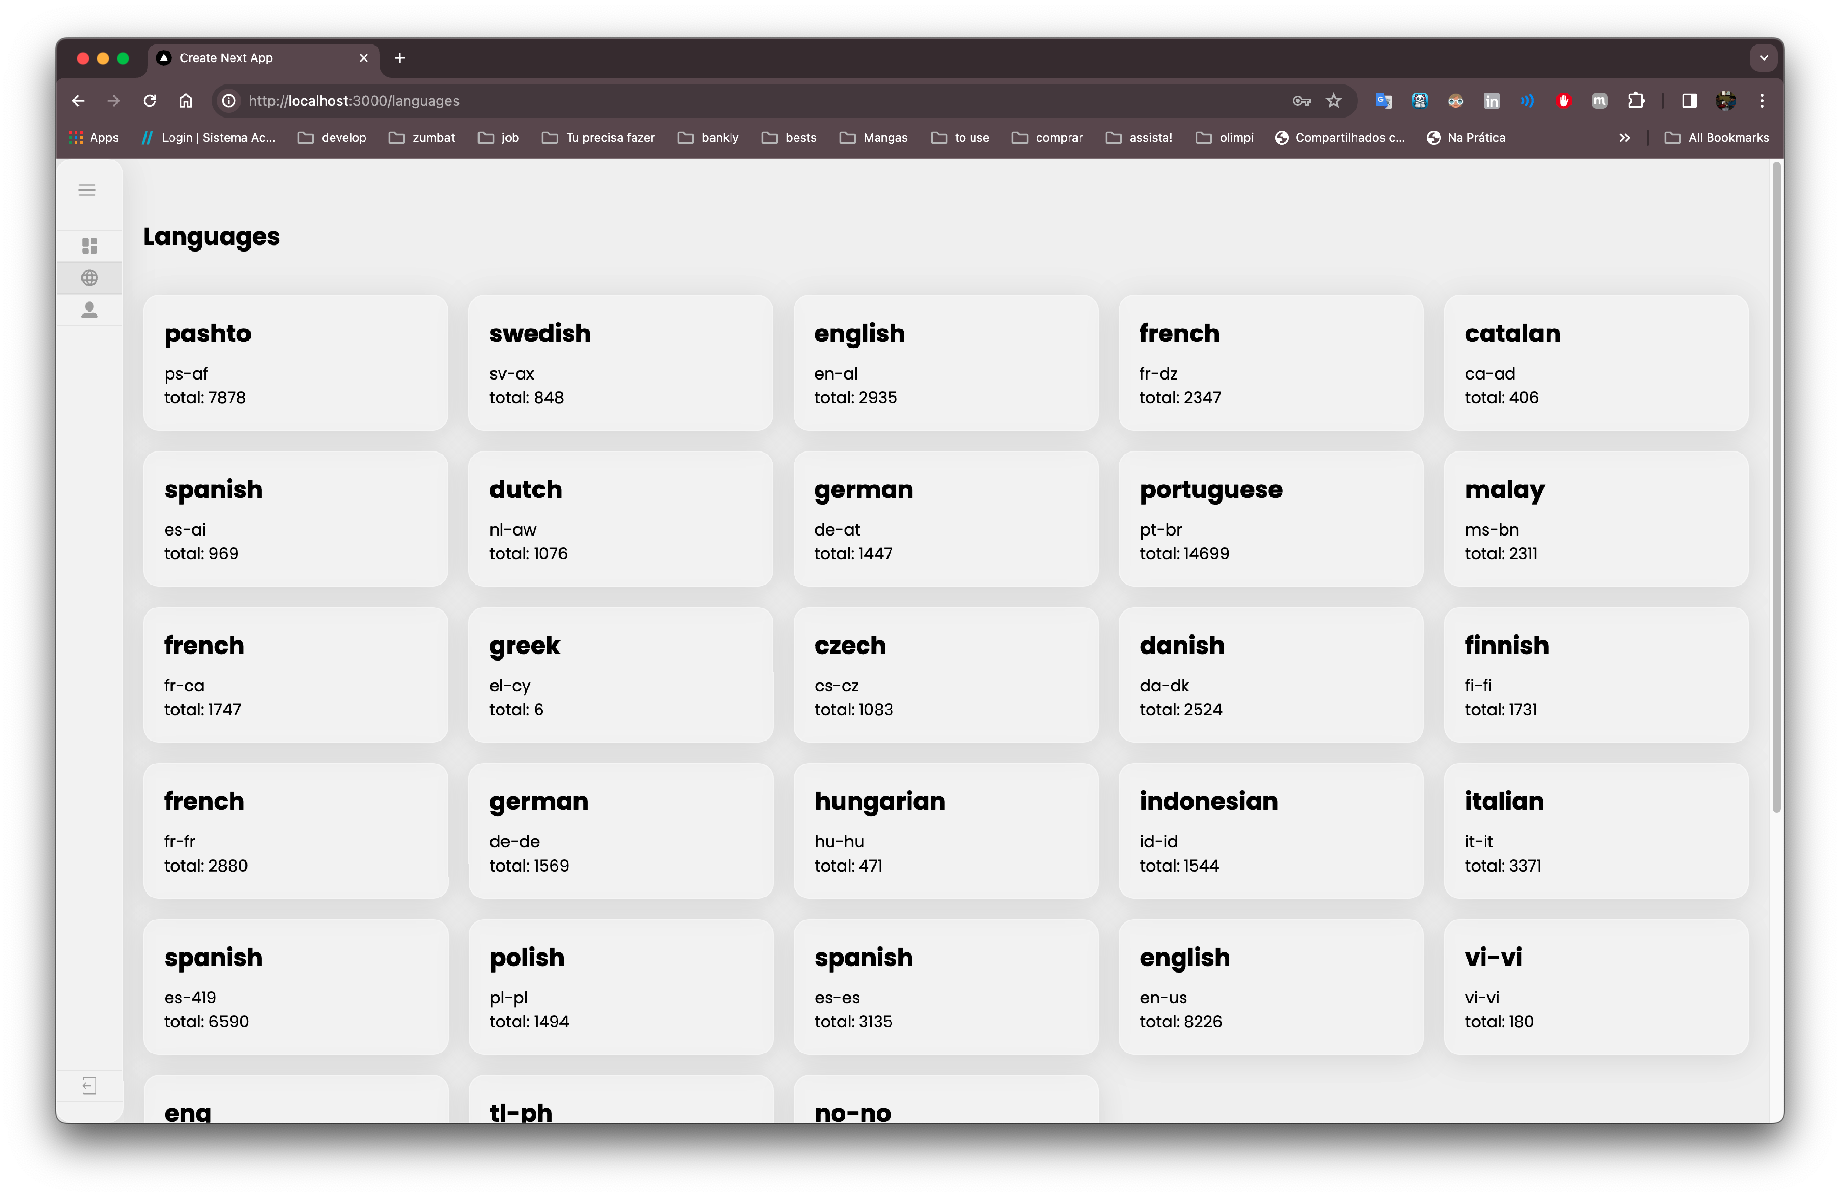
\includegraphics[width=1\textwidth]{assets/21.png}
      \end{minipage}
  \end{figure}
\end{frame}


\begin{frame}{}
  \begin{figure}[!h]
      \begin{minipage}[b]{0.5\linewidth}
        \centering
        \caption{
        The user profile with progress for each language.
        }
        \label{fig:site3}
        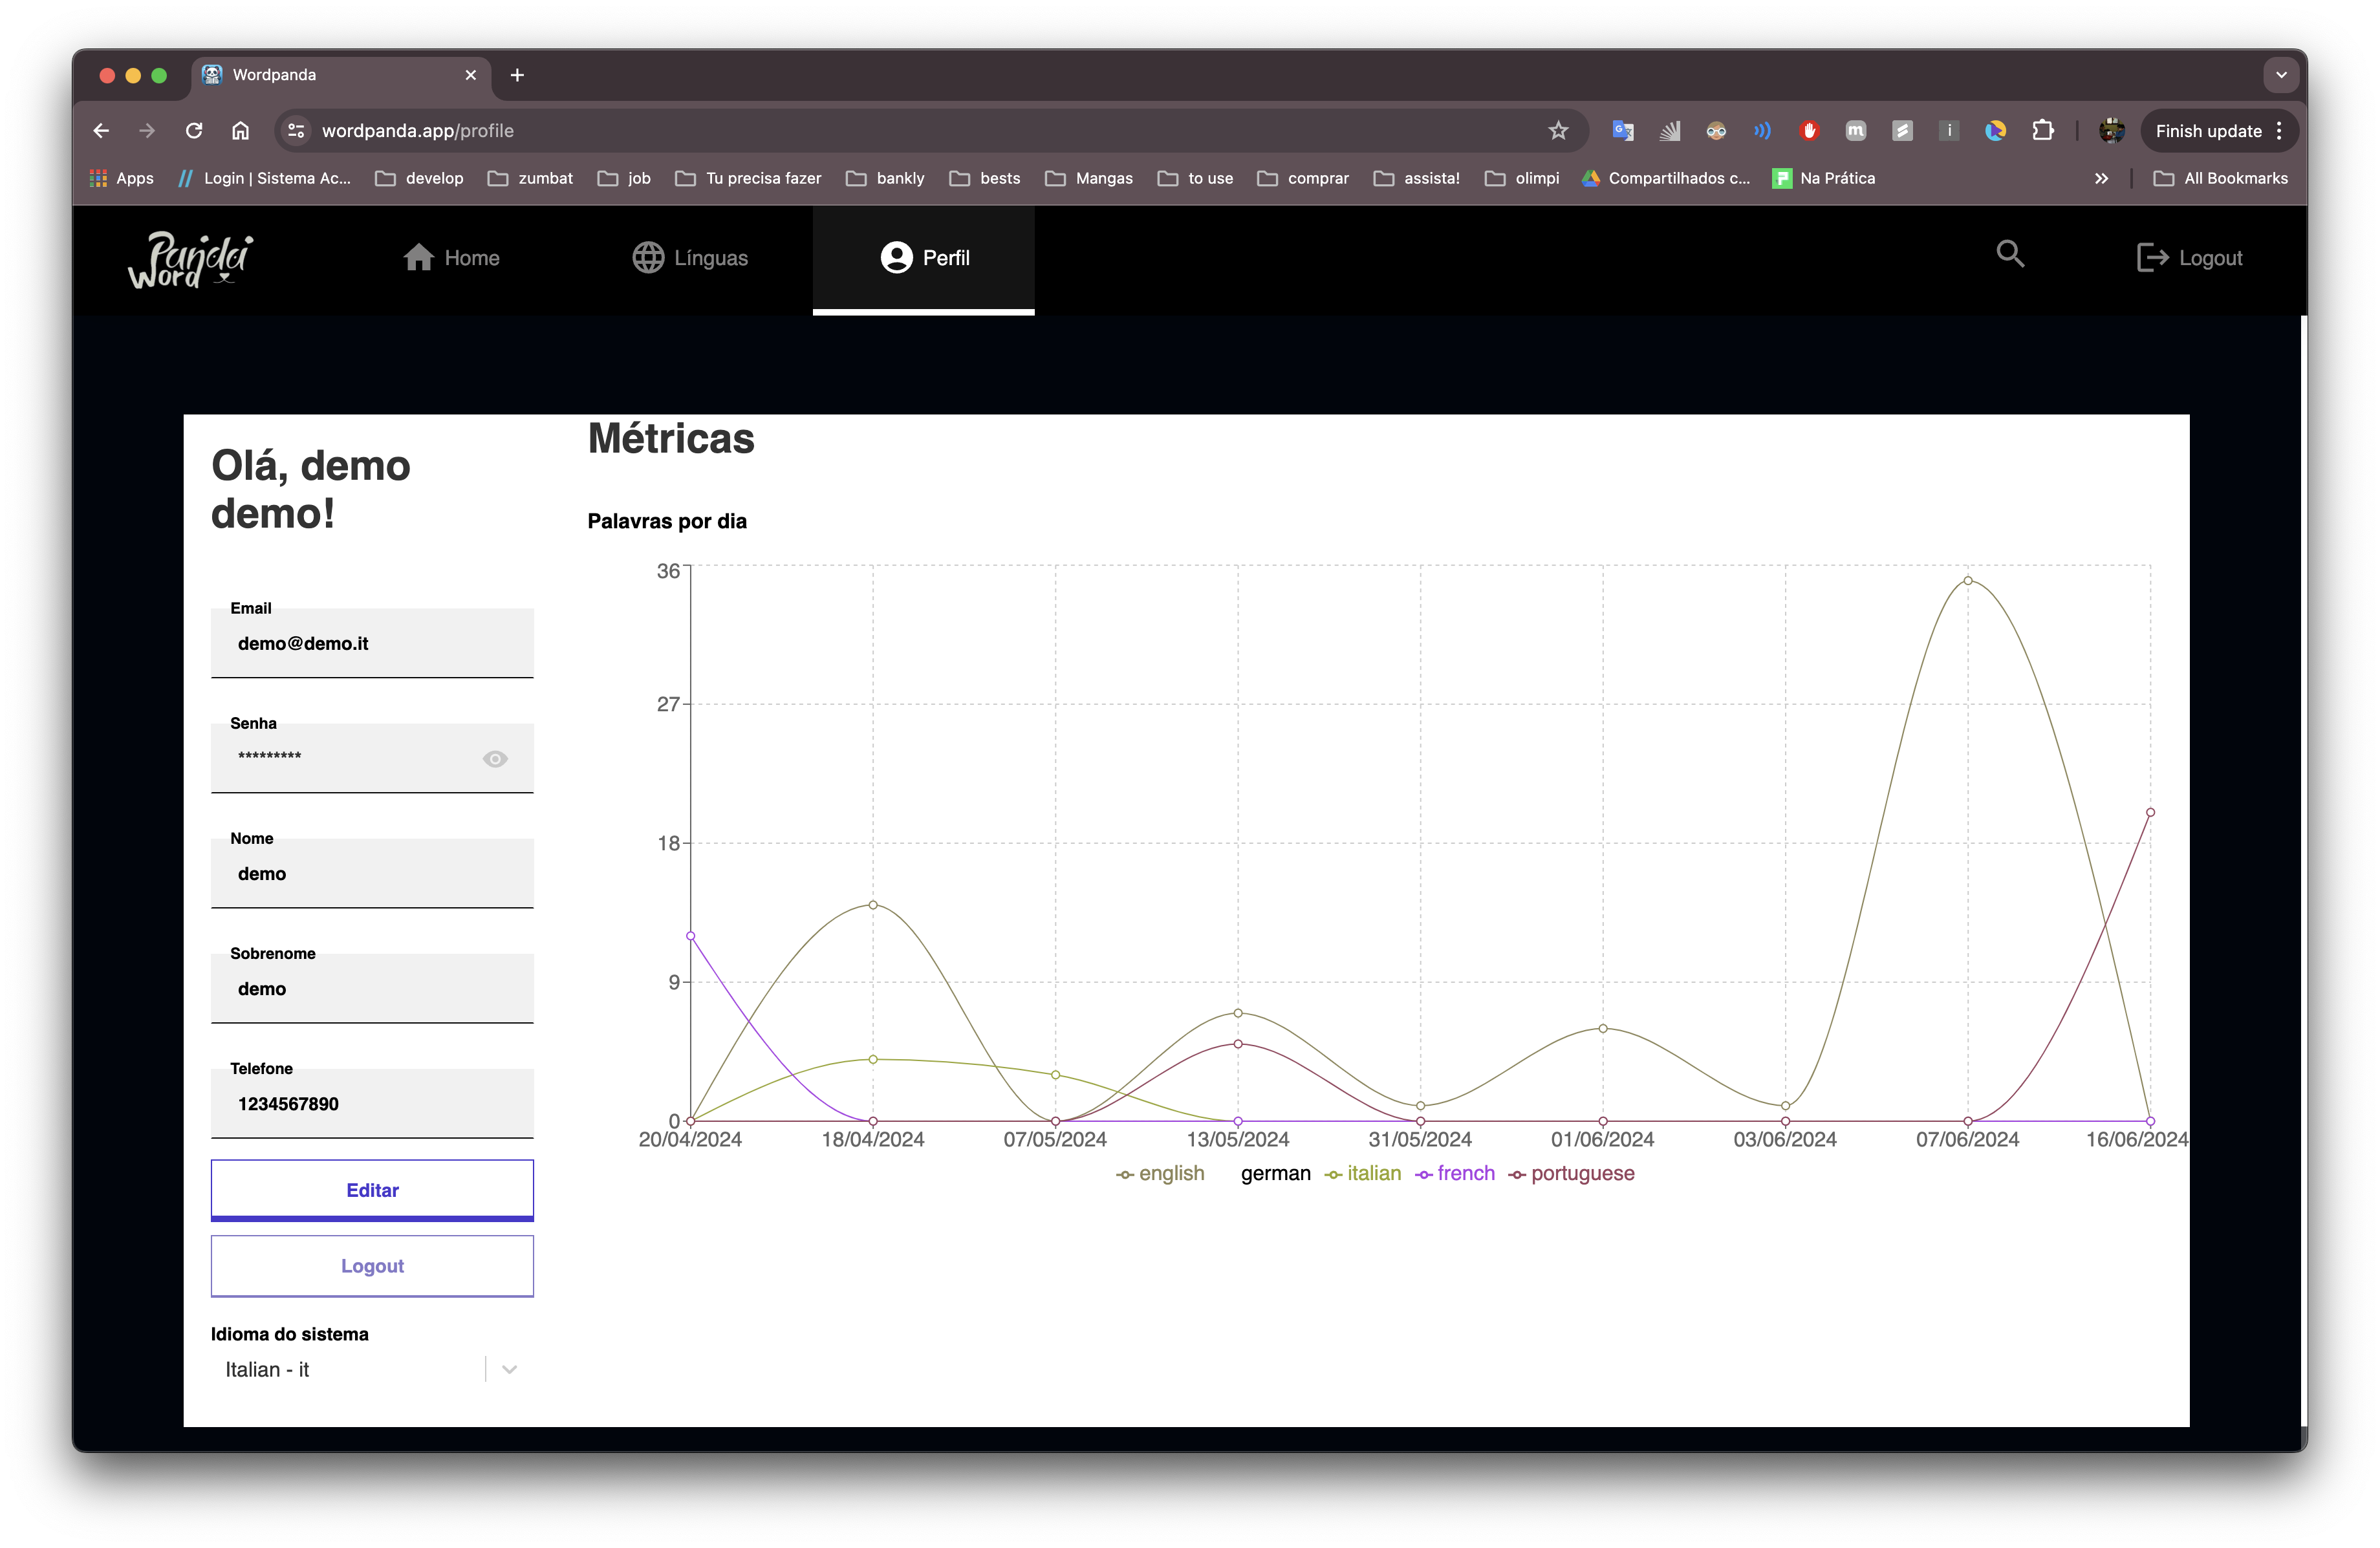
\includegraphics[width=1\textwidth]{assets/22.png}

      \end{minipage}
      \hspace{0.2cm}
      \begin{minipage}[b]{0.5\linewidth}
        \centering
        \caption{
        A list of languages when the user selects a language to learn.
        }
        \label{fig:site4}
        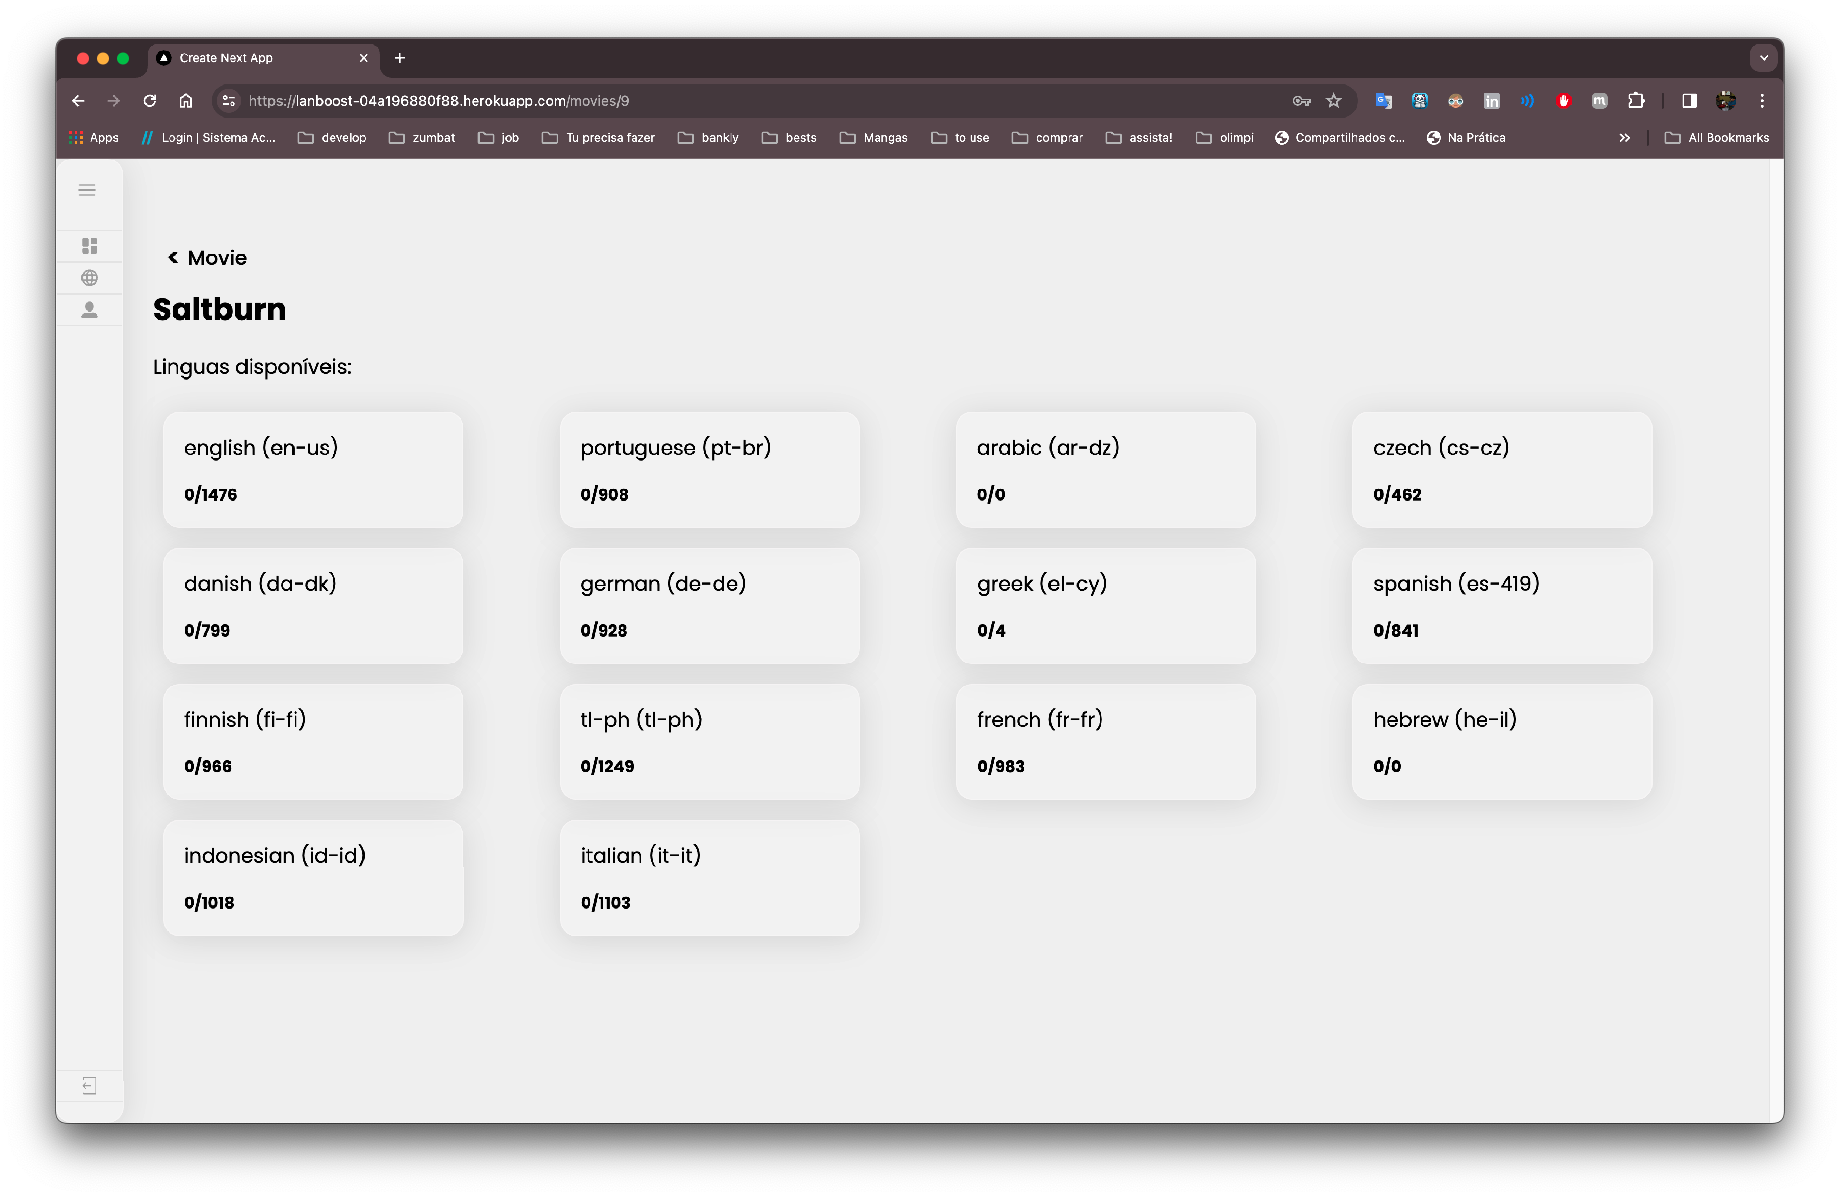
\includegraphics[width=1\textwidth]{assets/25.png}
      \end{minipage}
  \end{figure}
\end{frame}


    % \begin{figure}[h]
    %   \centering
    %   \caption{
    %   Example of the flashcard game 
    %   }
    %   \label{fig:site6}
    %   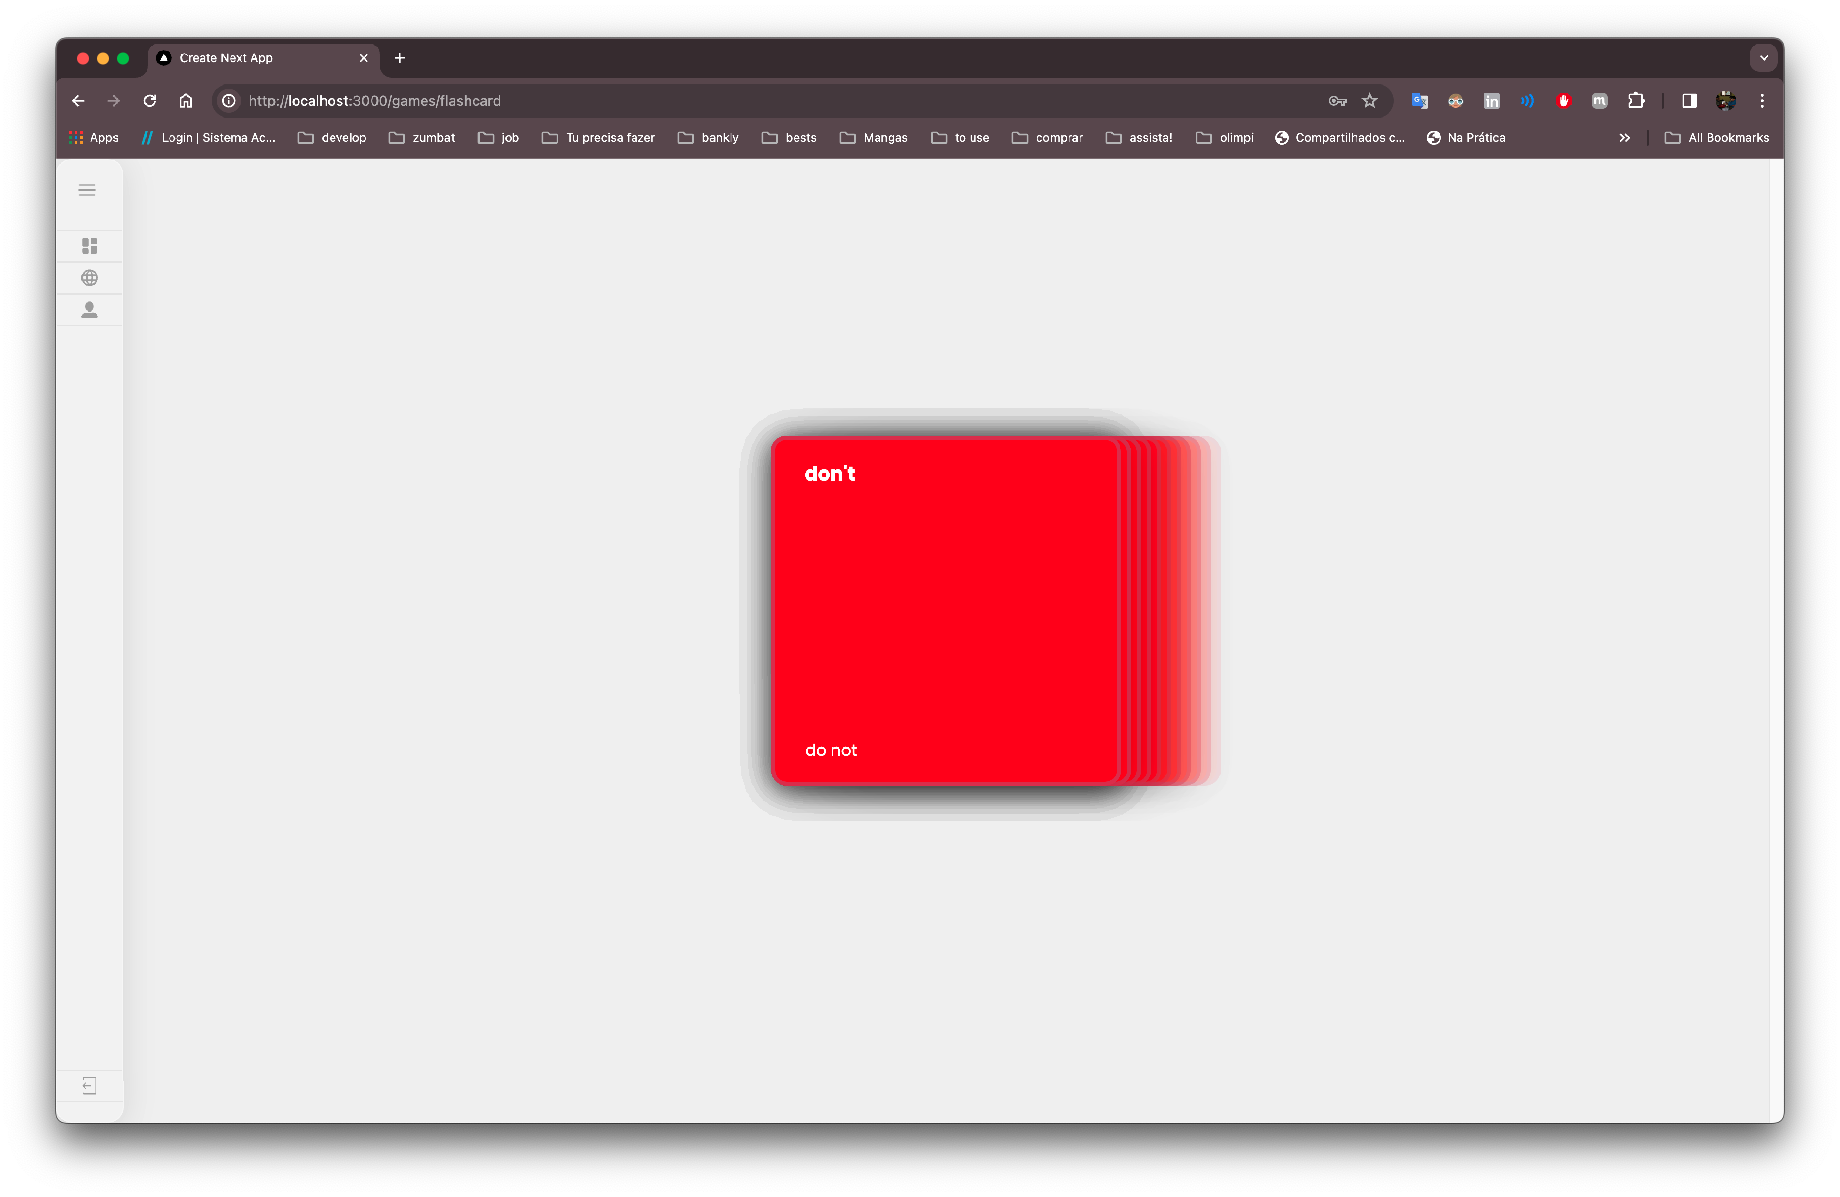
\includegraphics[width=0.8\textwidth]{assets/6.png}
    % \end{figure}


    % \begin{figure}[h]
    %   \centering
    %   \caption{
    %   Example of the Memory game 
    %   }
    %   \label{fig:site7}
    %   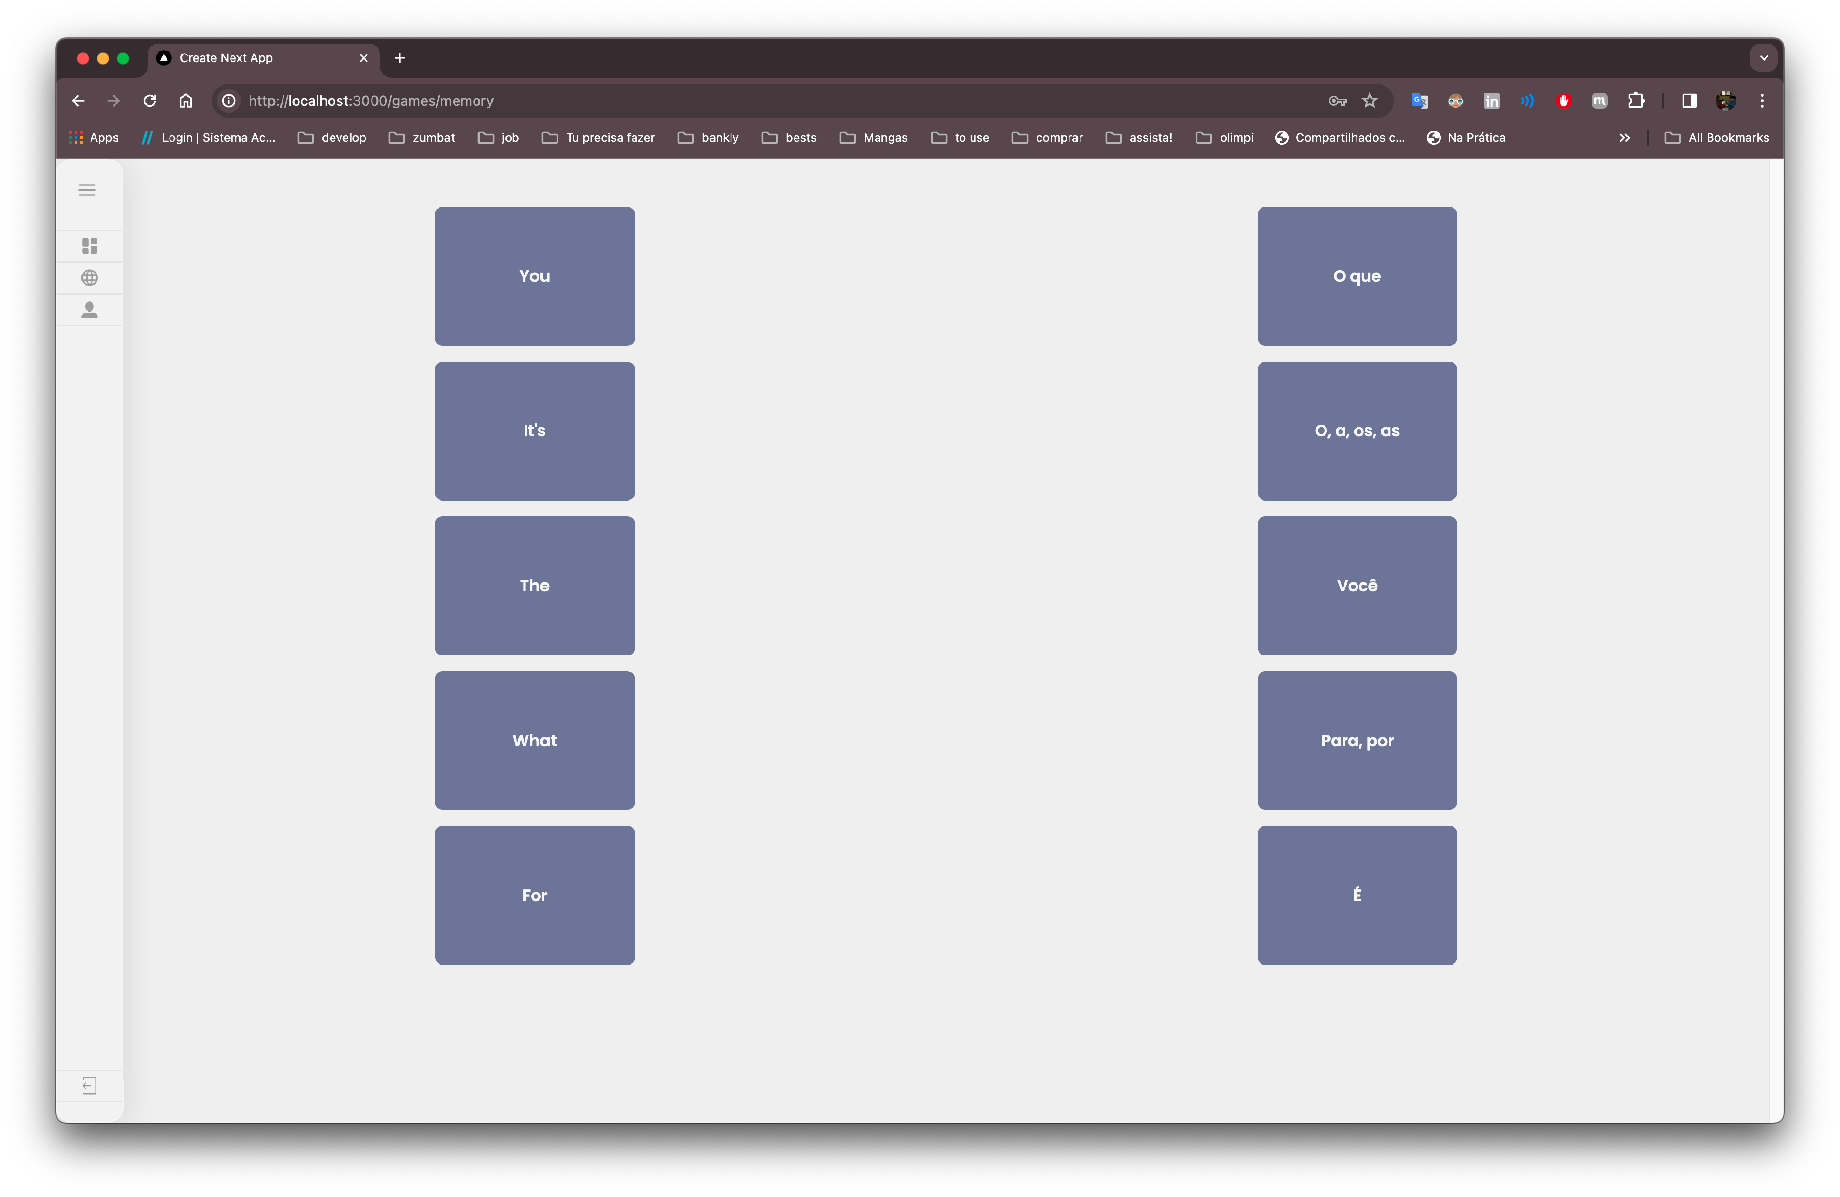
\includegraphics[width=0.8\textwidth]{assets/7.png}
    % \end{figure}

    % \begin{figure}[!h]
    %   \centering
    %   \caption{
    %   Example of the Quiz game 
    %   }
    %   \label{fig:site8}
    %   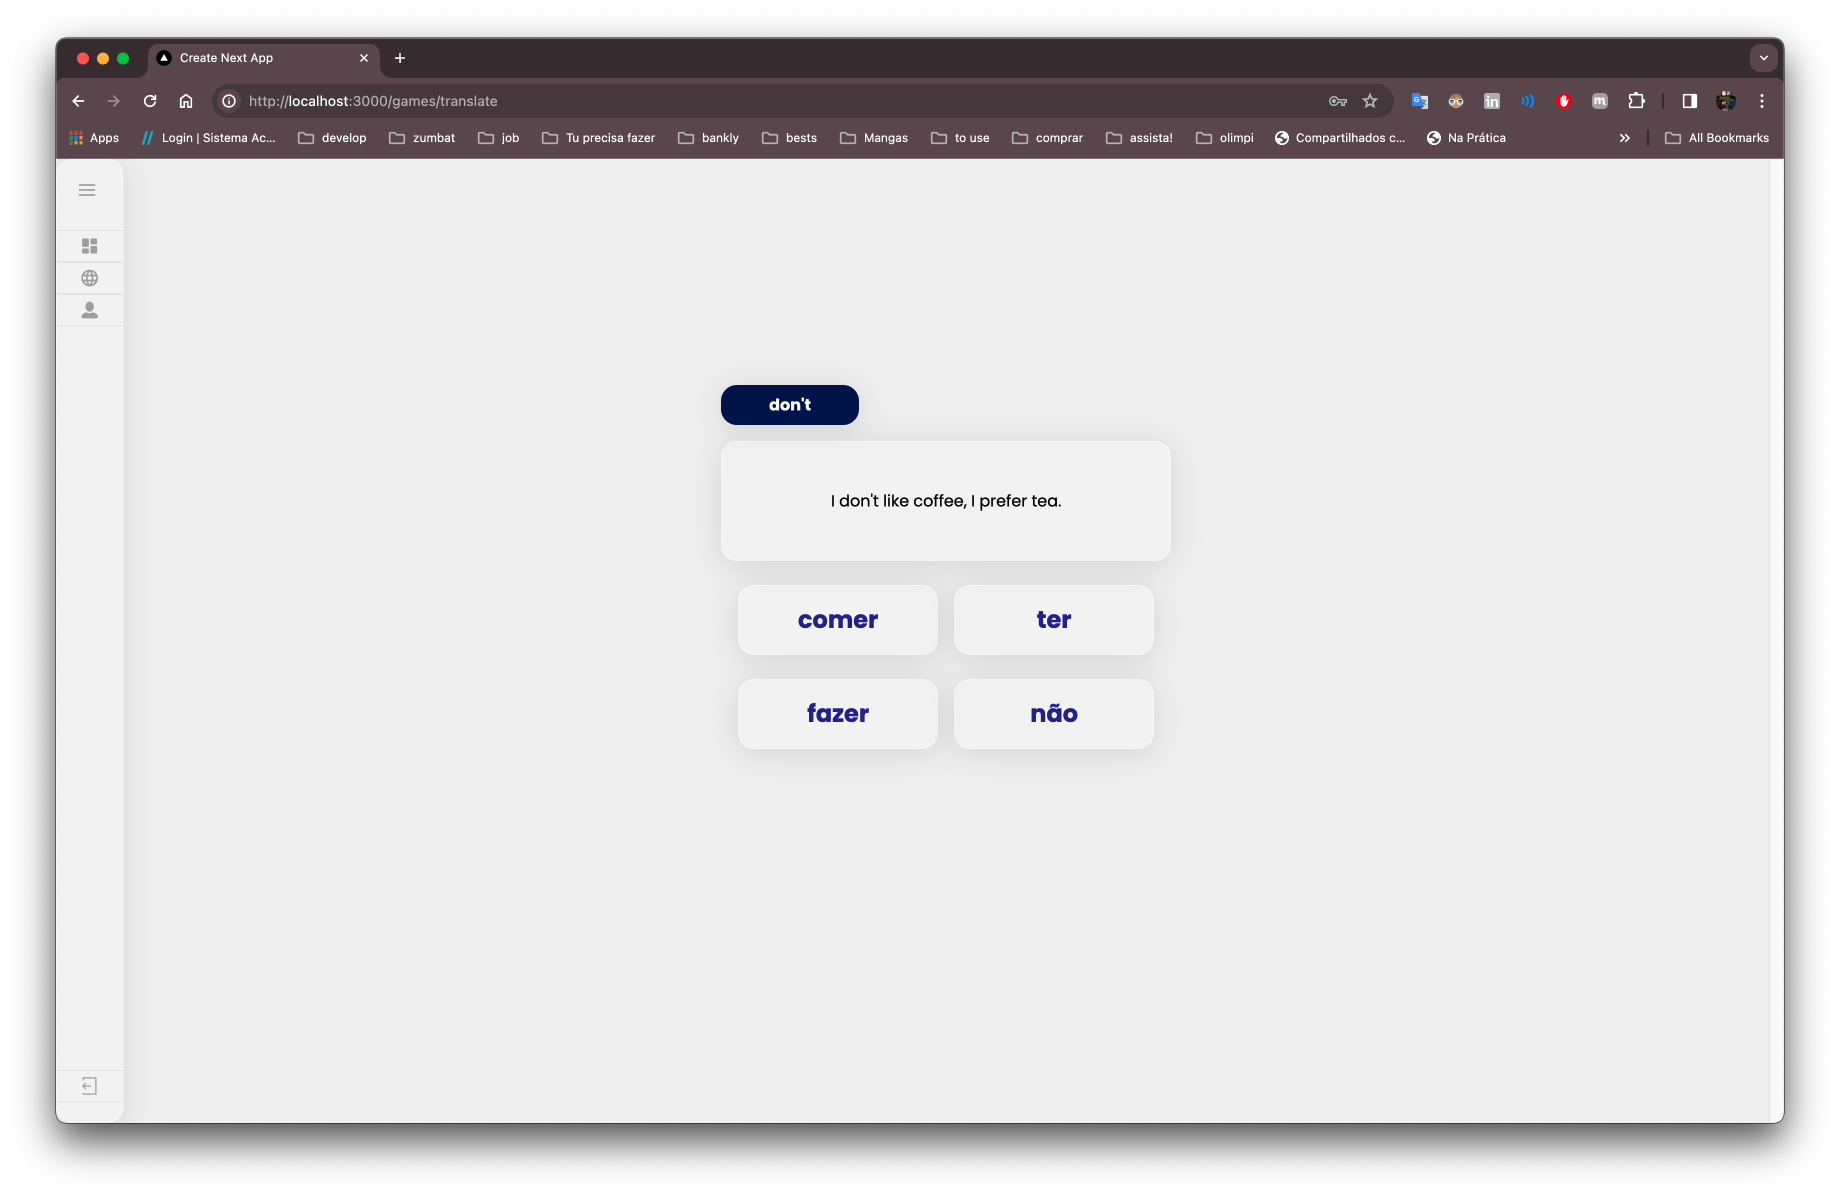
\includegraphics[width=0.5\textwidth]{assets/8.png}
    % \end{figure}
\subsubsection{iframe to extension}
      This module is used on a modal when the users open a movie on the streaming site. The user could interact with the application with the initial interface of site, but inside an iframe, where the user could select the gamer which he wants to play. 
      Those games are the Flashcard, Memory, and Quiz, as demonstrated in figure-\ref{fig:iframe2} figure-\ref{fig:iframe4}.
      The entire playing process is inside the iframe, and the user can interact with the application without leaving the streaming site.
      
      
    % \begin{itemize}
    % \item The list of games that the user can play;
    % , as demonstrated in the figure-\ref{fig:iframe1}.
    % \item The Flashcard, Memory and Quiz games, as demonstrated in the figure-\ref{fig:iframe2}, figure-\ref{fig:iframe3}, and figure-\ref{fig:iframe4}.
    % \end{itemize}


    % \begin{figure}[!h]
    %   \centering
    %   \caption{
    %   Games list inside iframe on the prime video site.
    %   }
    %   \label{fig:iframe1}
    %   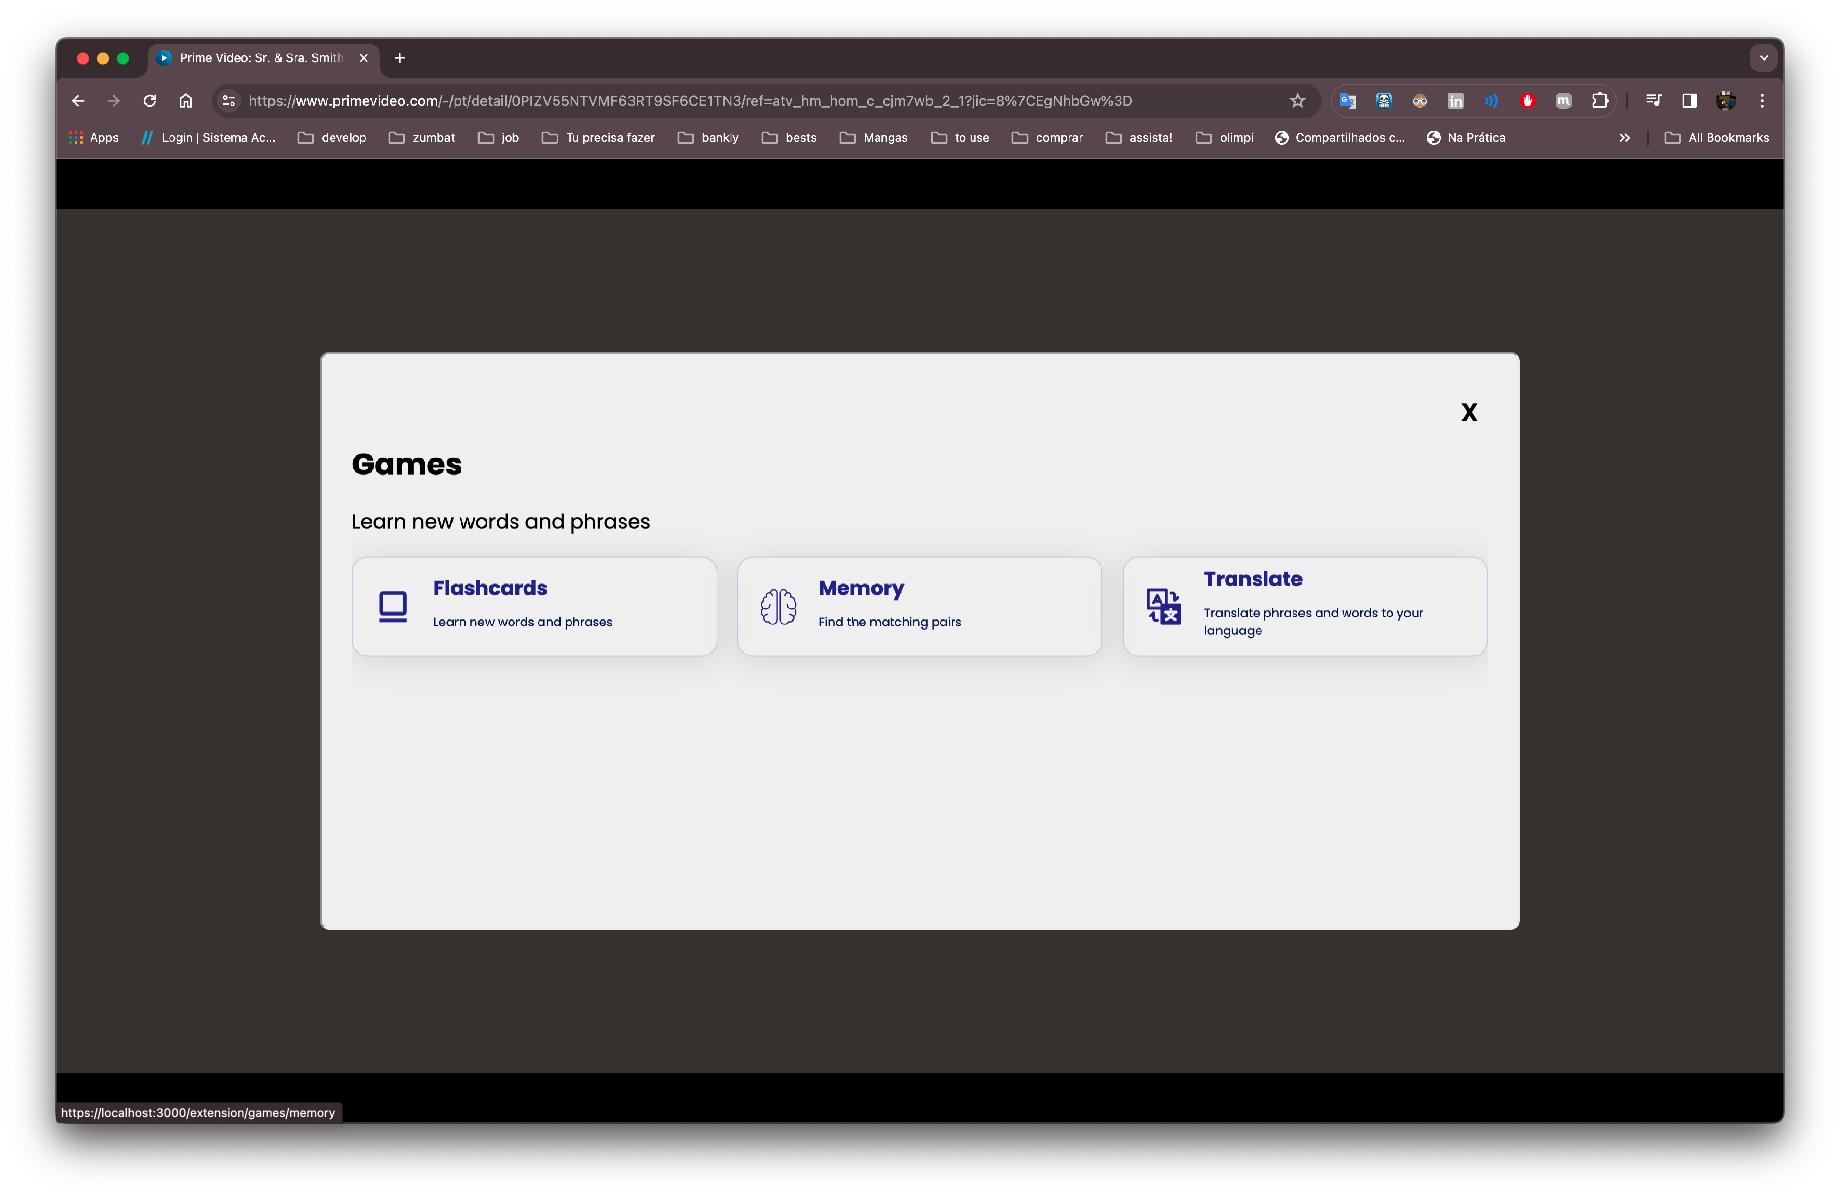
\includegraphics[width=0.45\textwidth]{assets/9.png}
    % \end{figure}


    \begin{frame}{}
      \begin{figure}[!h]
          \begin{minipage}[b]{0.5\linewidth}
            \centering
            \caption{
            Games Flashcard inside iframe on the prime video site.
            }
            \label{fig:iframe2}
            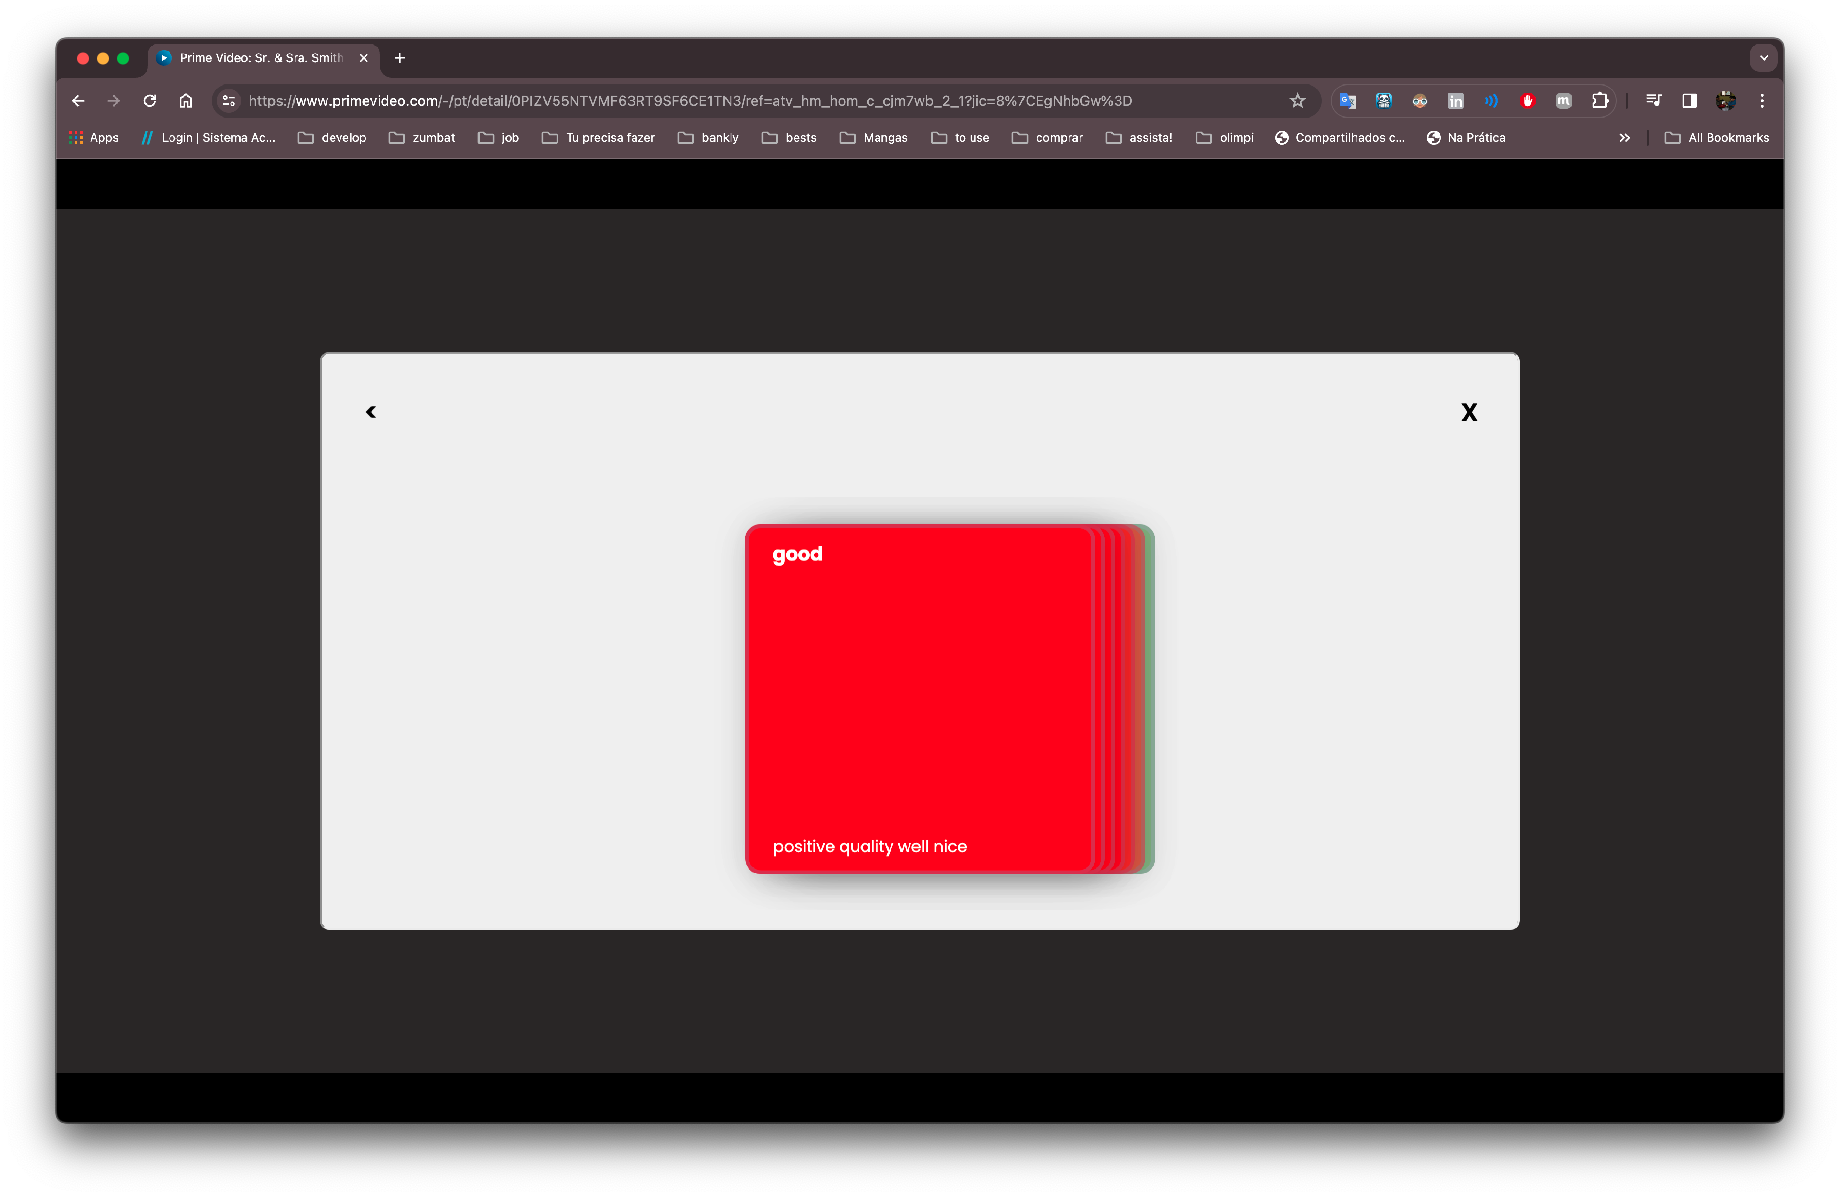
\includegraphics[width=1\textwidth]{assets/10.png}
          \end{minipage}
          \hspace{0.2cm}
          \begin{minipage}[b]{0.5\linewidth}
   
  
            \centering
            \caption{
            Games Translate inside iframe on the prime video site.
            }
            \label{fig:iframe4}
            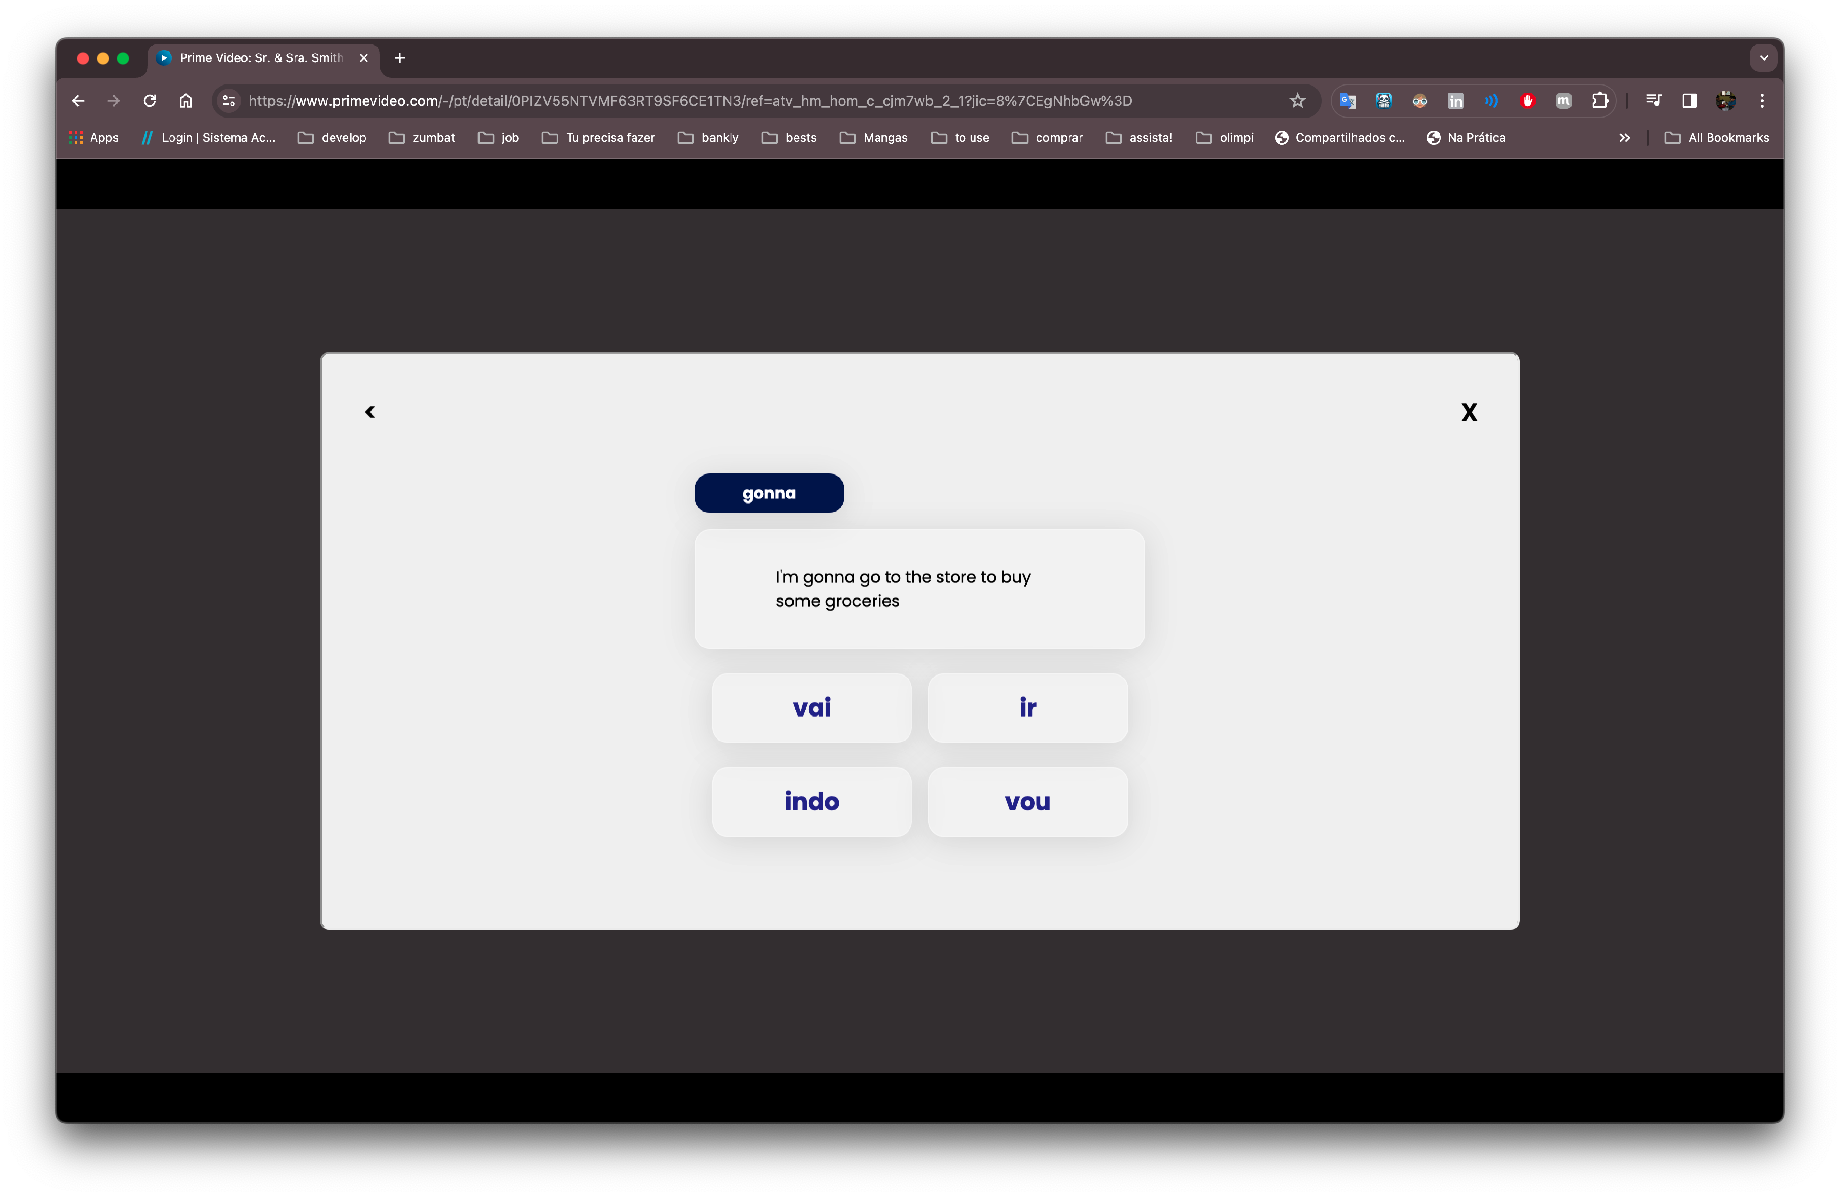
\includegraphics[width=1\textwidth]{assets/12.png}
          \end{minipage}
      \end{figure}
    \end{frame}


\subsubsection{iframe to app}
This module is used by the app but also used on the pop-up of the extension. This provides a small interface and resizes components to adapt to that environment. Examples of ways to interact with the application with the following interfaces:
\begin{itemize}
  \item Home Page:  that screen provides a list of languages and movies as demonstrated in the figure-\ref{fig:app2}.
  \item Language by movie page: list all languages for each movie as demonstrated in the figure-\ref{fig:app5}.
  \item Game Translate Page: A game where the user needs to inform the correct translation for a word in a specific phrase demonstrated in the figure-\ref{fig:app6}.
  \item And the other games as the site and iframe extension. 
  \end{itemize}
  



  \begin{frame}{}
    \begin{figure}[!h]
        \begin{minipage}[b]{0.31\linewidth}
          \centering
          \caption{
          List of languages and movies inside iframe on the app.
          }
          \label{fig:app2}
          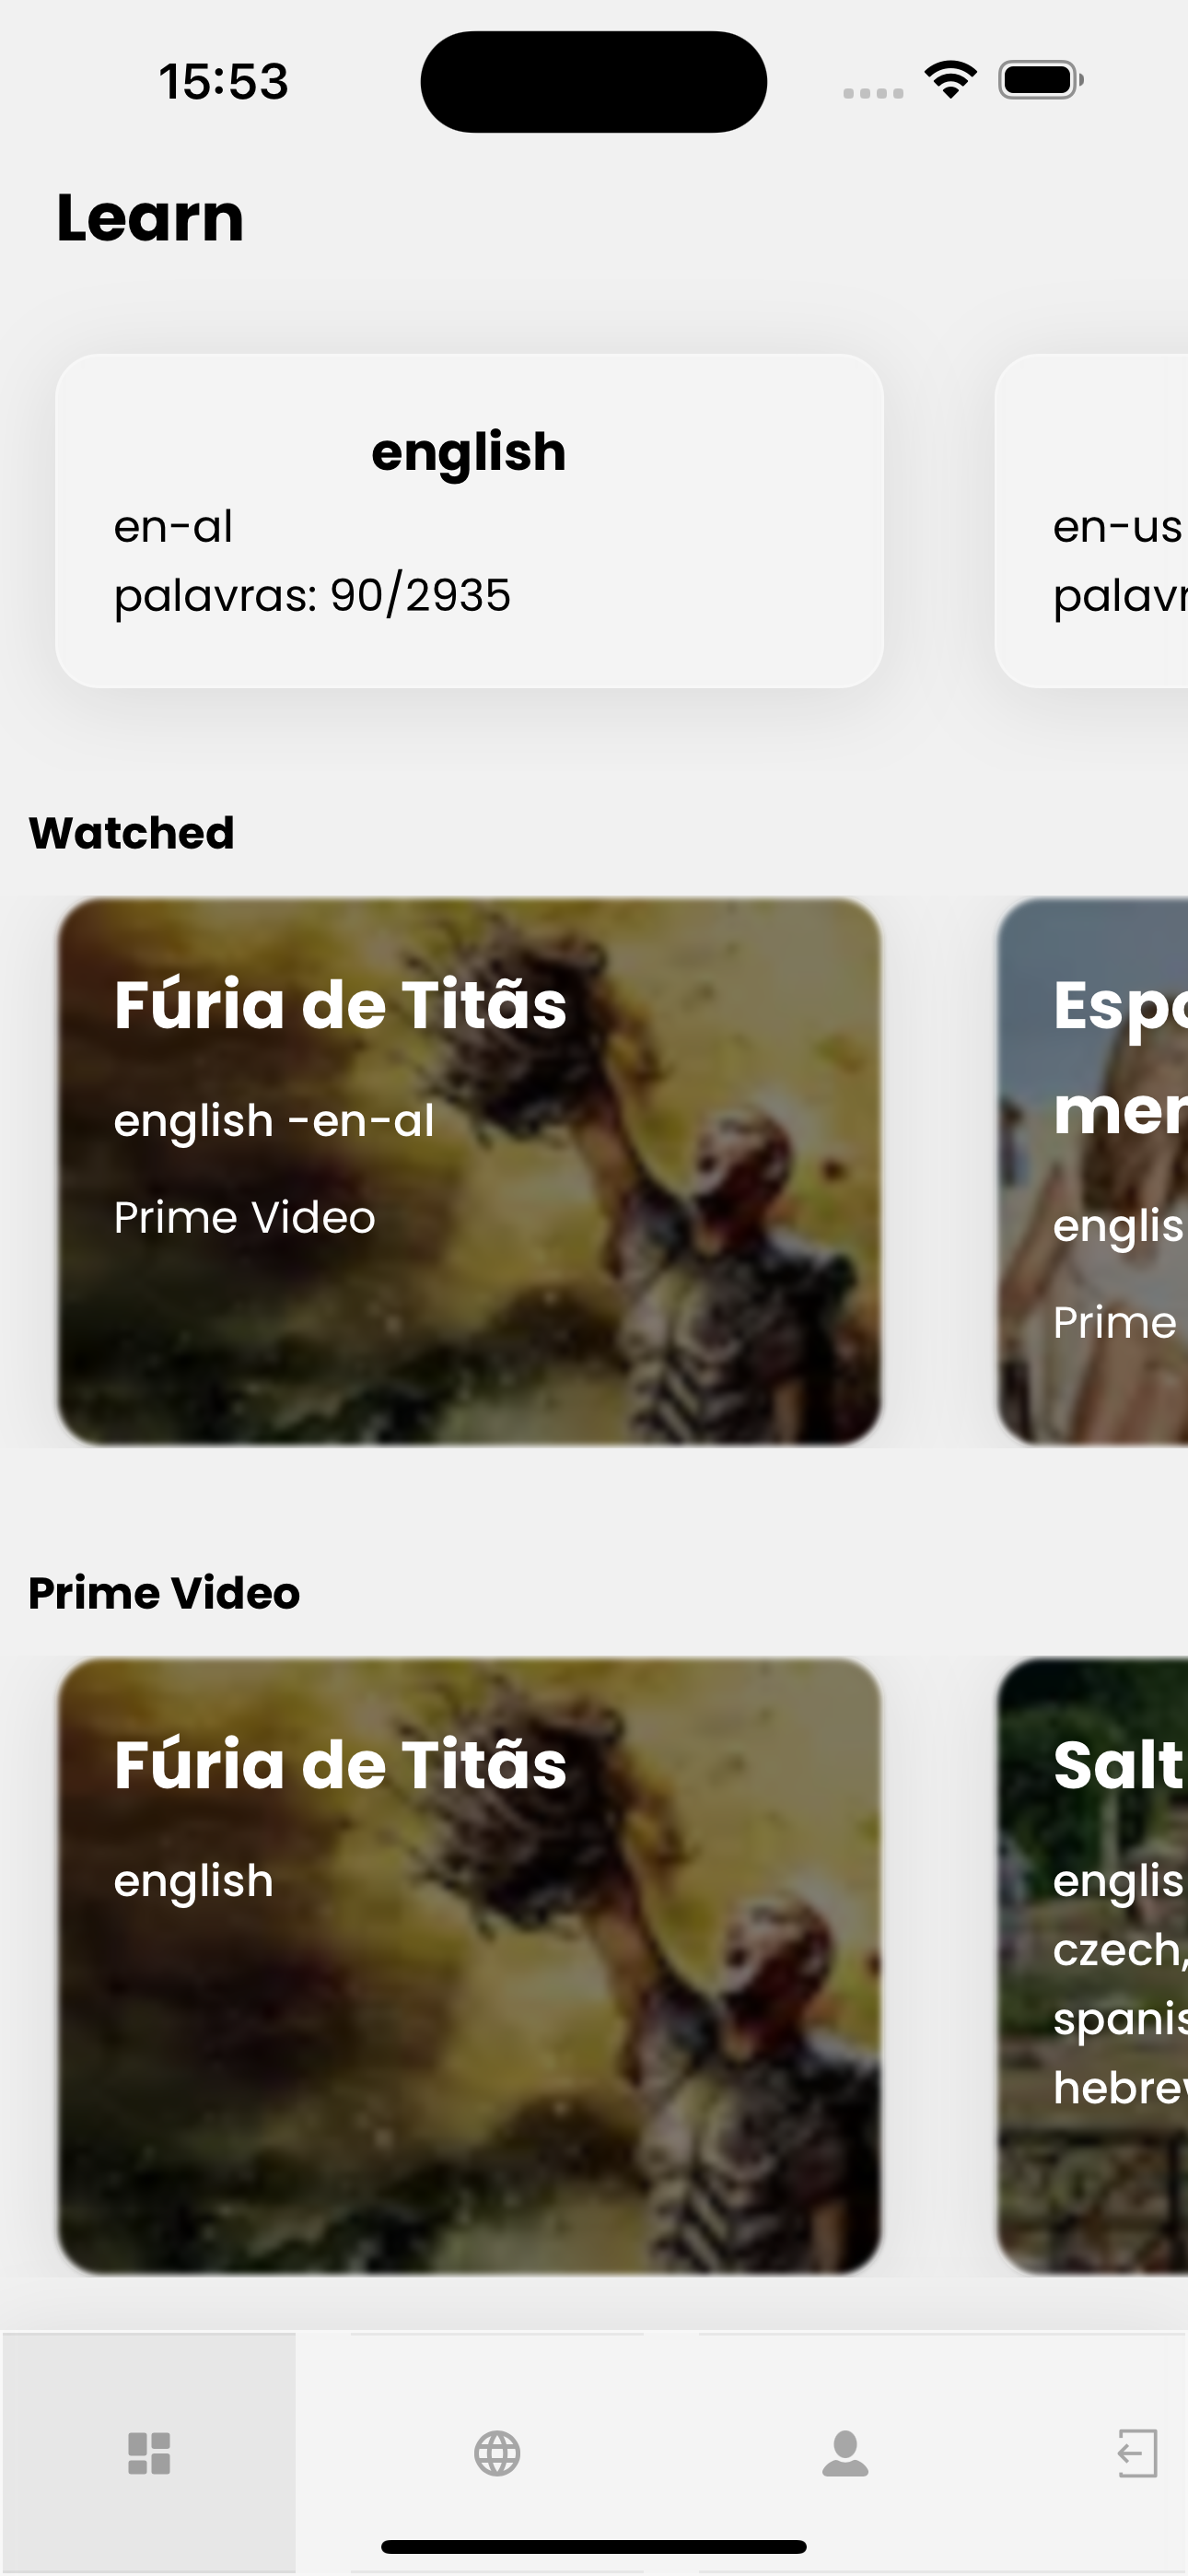
\includegraphics[width=0.7\textwidth]{assets/15.png}
        \end{minipage}
        \hspace{0.1cm}
        \begin{minipage}[b]{0.31\linewidth}
          \centering
          \caption{
           List of languages by movie inside iframe on the app.
          }
          \label{fig:app5}
          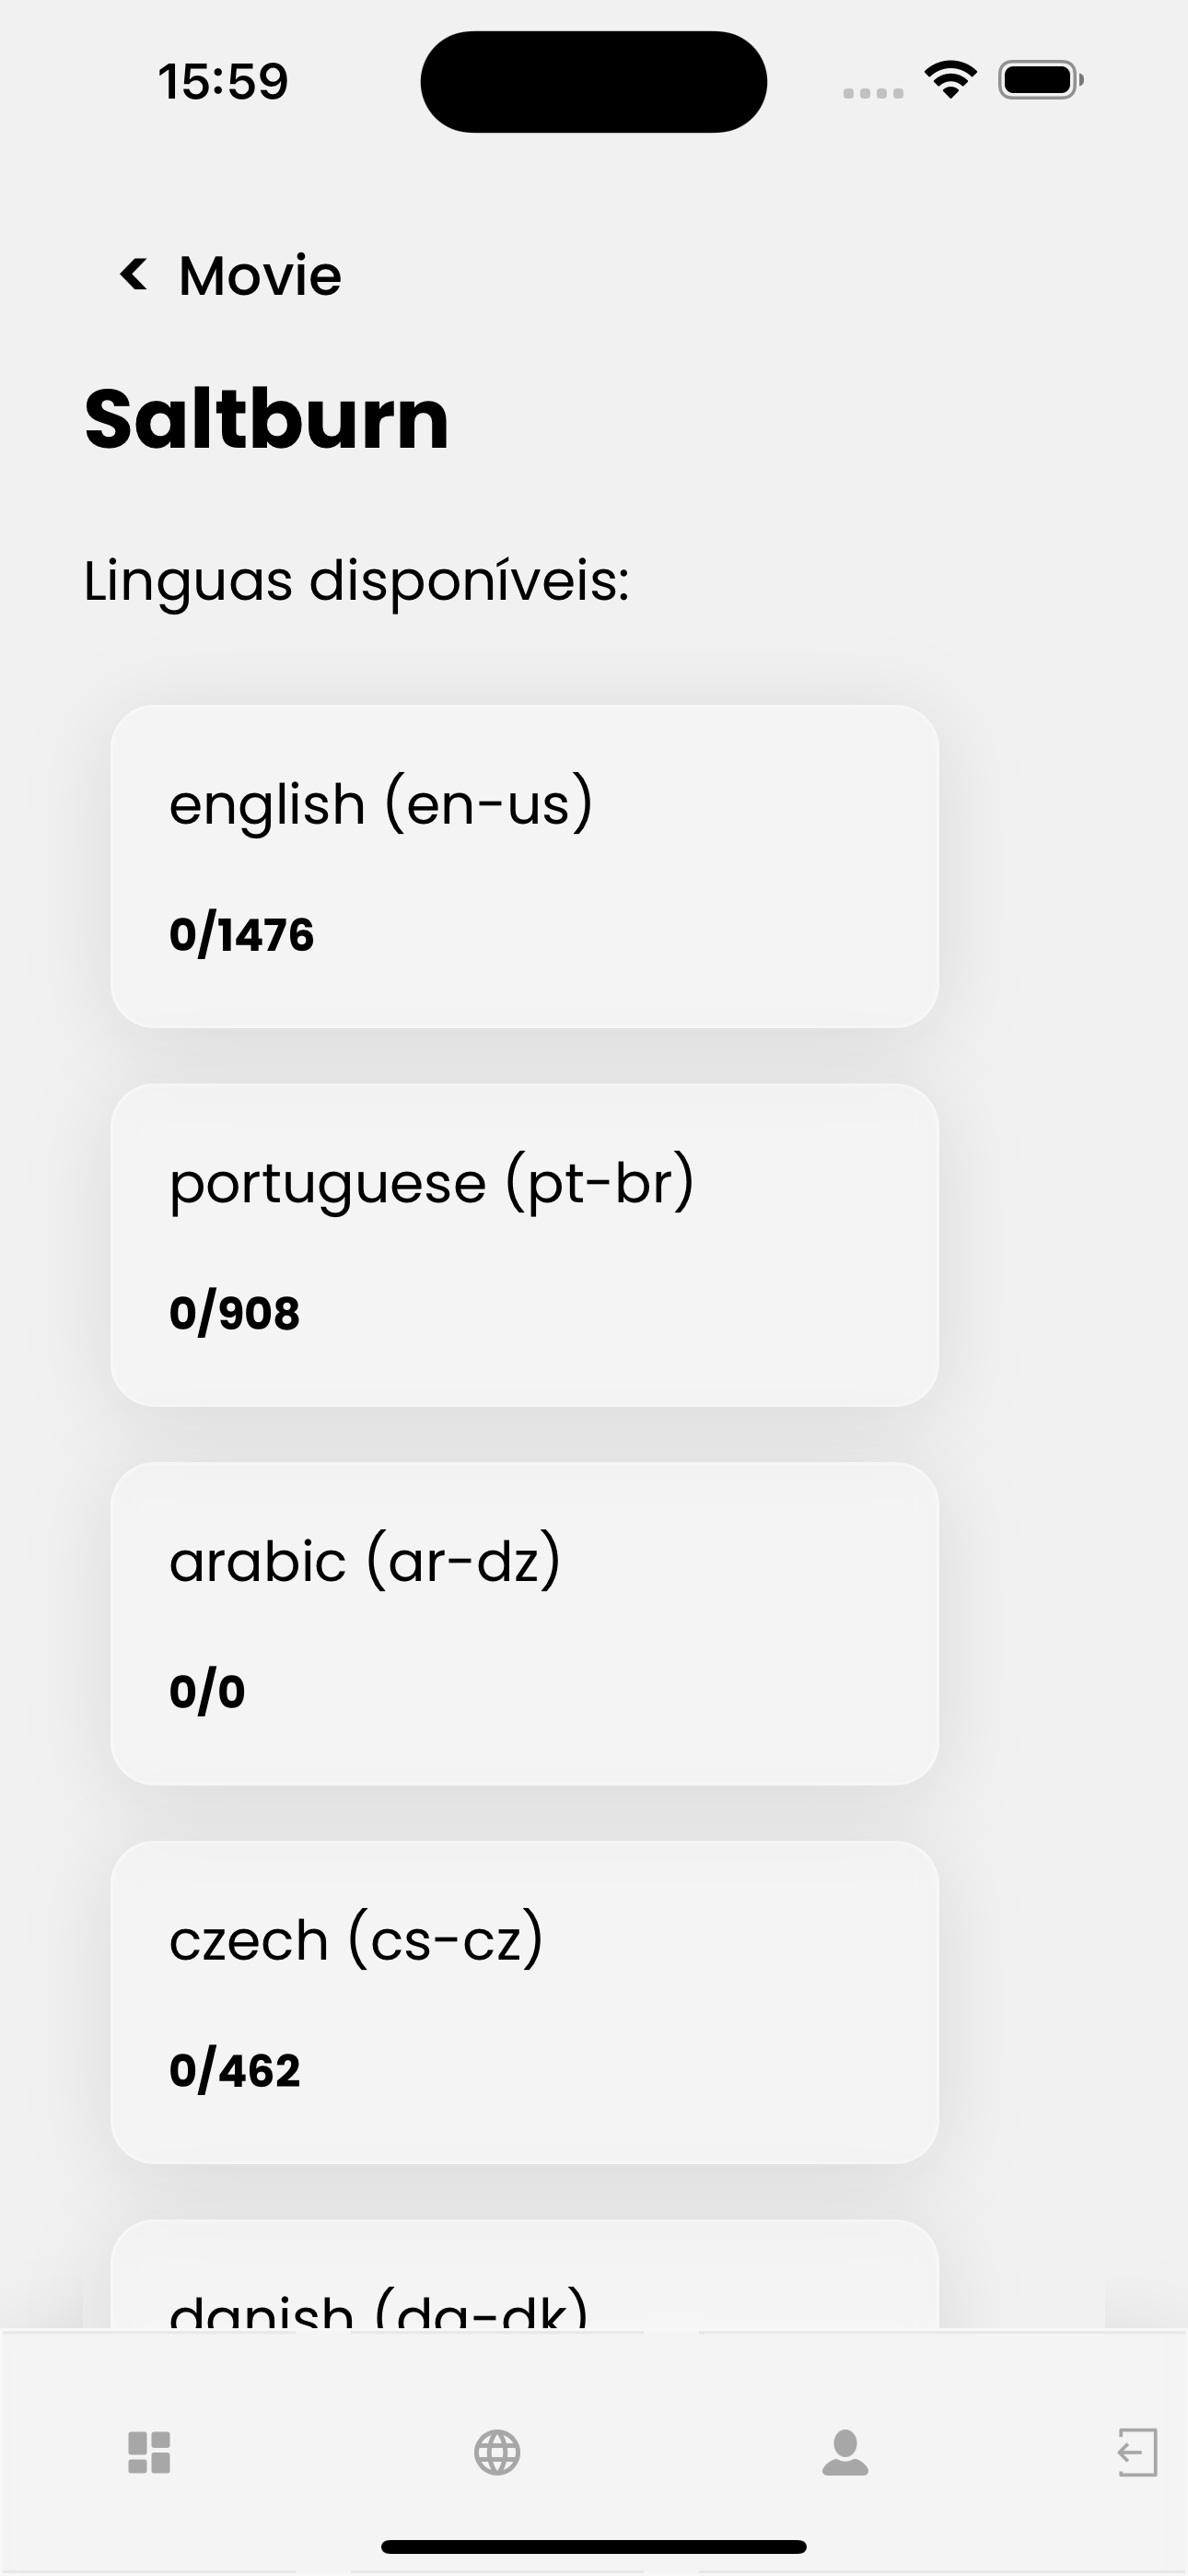
\includegraphics[width=0.7\textwidth]{assets/18.png}
        \end{minipage}        
        \hspace{0.1cm}
        \begin{minipage}[b]{0.31\linewidth}
          \centering
          \caption{
           Translate game inside the the iframe on the app.
          }
          \label{fig:app6}
          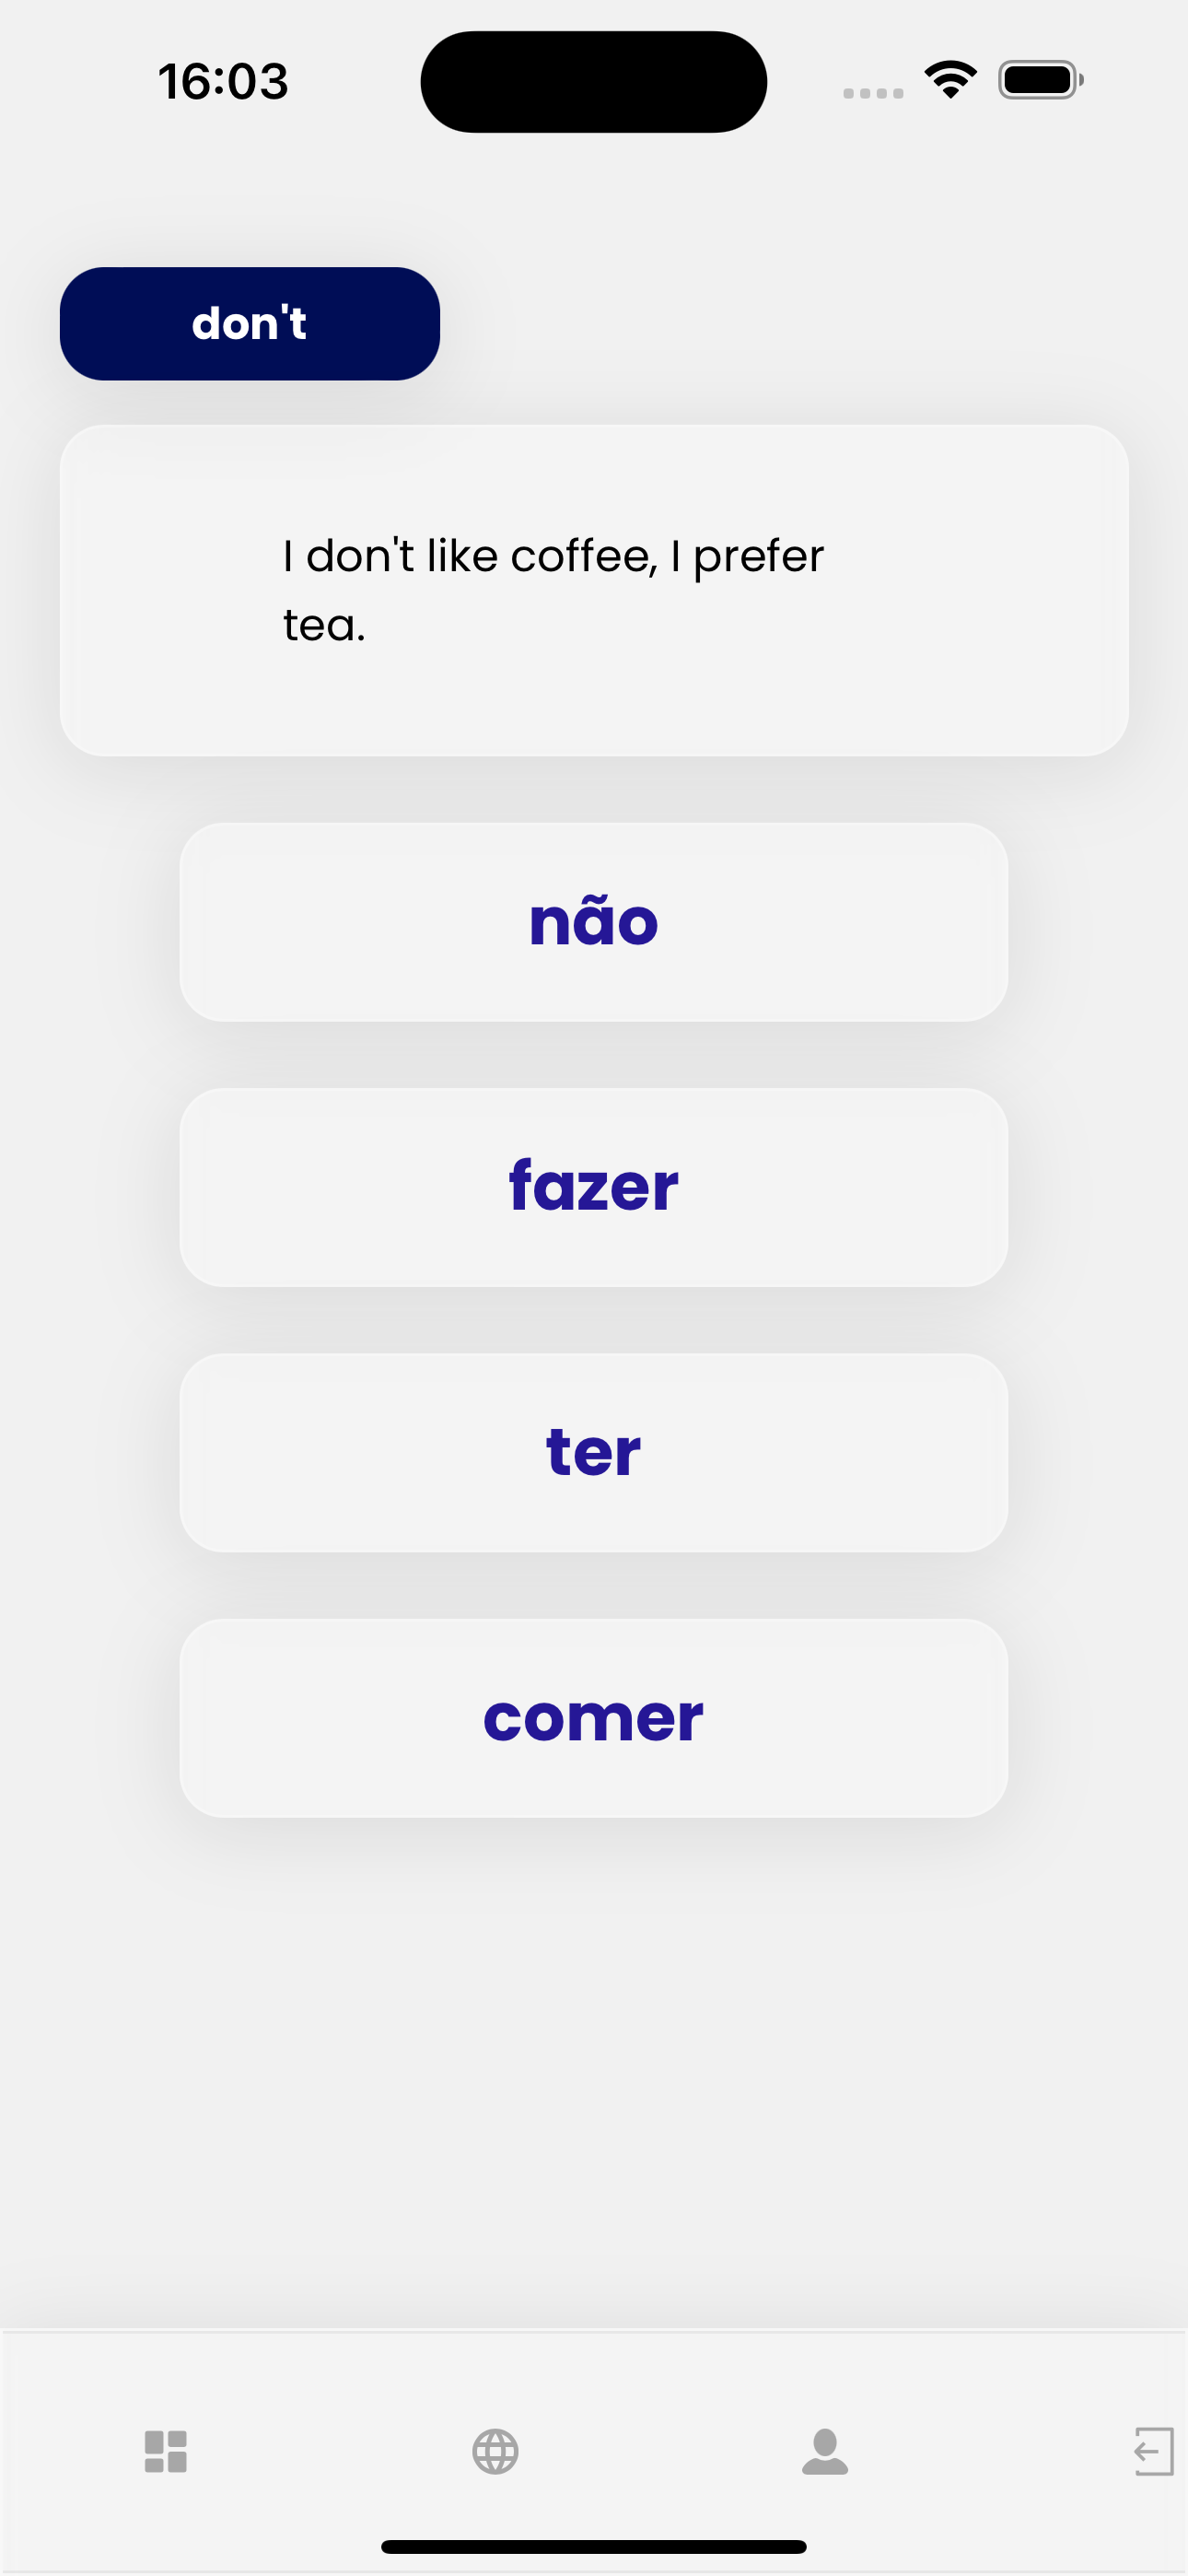
\includegraphics[width=0.7\textwidth]{assets/19.png}
        \end{minipage}
    \end{figure}
  \end{frame}





\subsection{Future Improvements}

For future improvements, there are subsections for each one and each environment (extension, site, app, backend, and AI) to improve the prototype. Because this work is a prototype, the goal is to improve the user experience and the learning process,  make the application more responsive and fast, create a better interface, improve the user experience, and reduce costs to maintain the application.

\subsubsection{Extension}
The extension needs to be some refactors to turn more responsible and fast, because the background service that takes the subtitles is slow and executes a cron-job to get the subtitles. Is necessary to study ways to do this using dispatch events and workers. \\
Currently, the repertoire of sites is so small that the extension could communicate, and restrict only to Prime video, but the goal is to expand to other platforms like Netflix, Disney+, and others. \\
Also is important to create a WebSocket to extract pieces of information from the site, considering that some streaming uses another technology to show the subtitles. \\
Considering that is possible to create communications between extensions or sites, a discussion about the possibility of integrating with other tools like Language Reactor, is viable.


\subsubsection{Site}
The site is the core of the application and is necessary to improve the user experience and make it more responsive. The site will be expanded to include new features like interactive exercises and games to reinforce vocabulary acquisition. \\
About the games, is necessary to create a better interface and improve the user experience. Because the games are the part visible at the core of the learning process, the user needs to have a good experience to continue using the application. The site was created without a professional designer, and games are the part that needs more attention in design. \\
The entire site needs to be more responsive and fast so that the user can understand and use it without any problems. The UX is missing, and the site needs to be redesigned. \\
Levels, interests, and other user information are not being used to improve the user experience, and the site needs to be customized to the user's level and interests, providing an interactive and engaging learning environment. \\
The last part about UX is the current language of the site, which is not possible to change the site language and is a relevant part of improving the user experience. \\
More about technology is interesting to associate the site with the WebSockets also, and create new channels to communicate with mobile and notify the user to study like a reminder. 
\subsubsection{App}
The app will be improved to capture device information and send it to the iframe to make it more responsible and fast. This possibility sends to the backend that information and creates a dashboard or extract to discover the user behavior and how to improve it. \\
The channel to communicate with the site to possibly configure notifications is also an important feature, because a huge part of the users use the app to study, and the app needs to remember the user to do this. 
\subsubsection{Backend} 
On the backend, the API routers will be improved using workers because the data will be extensive, and the app and site will be faster and more responsive. \\
Some API routers will be improved using workers because the data will be extensive, and the app and site will be faster and more responsive. \\
As the data of each word is a complex process a solution is to build routines to run at night that will recalculate the user progress and the word level based on the results of all users.
Another important part is the language manager, that will be changed using only the language name, not the language code. \\
And the last part is the web sockets, which will be created to improve communication between the extension and the site, and the site and the app. 

\subsection{AI}
The AI of choice is the gpt-3.5-turbo-1106 model developed by OpenAI, incurring costs of \$0.0010 per 1K tokens of input and \$0.0020 per 1K tokens of output. The goal is to reduce costs. Enhance prototype performance and stabilize monthly payments by leveraging proprietary AI technology. Considering the adoption of Smaug-72B-v0.1, an advanced open AI model known for surpassing the capabilities of my current paid AI solution. The transition to utilizing in-house AI will occur when it becomes more advantageous than relying on third-party APIs.
\subsection{MVP}
The application was publicly released on the website and the extension was published on the Chrome Web Store. The application is available for users to download and use. The application is currently in the MVP stage, with basic features and functionality. The MVP includes the features previously mentioned. \\
The MVP is a prototype that demonstrates the potential of using technology to facilitate language learning. The MVP is a proof of concept that showcases the core functionality of the application. The MVP is a starting point for future development and improvements. 


\begin{frame}{}
  \begin{figure}[!h]
      \begin{minipage}[b]{0.5\linewidth}
        \centering
        \caption{
        Database data of words, attempts and movies
        }
        \label{fig:database_data}
        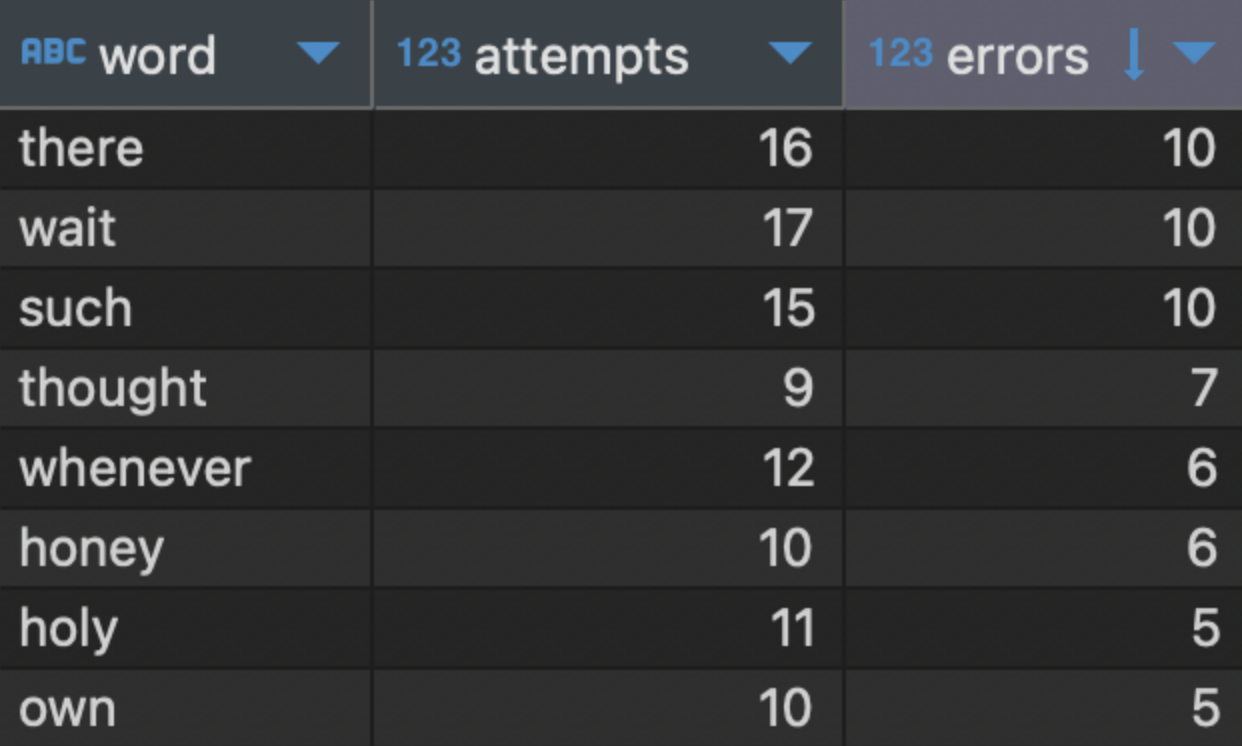
\includegraphics[width=1\textwidth]{assets/32.png}
      \end{minipage}
      \hspace{0.1cm}
      \begin{minipage}[b]{0.5\linewidth}

        \centering
        \caption{
        Words with the most errors
        }
        \label{fig:database_errors}
        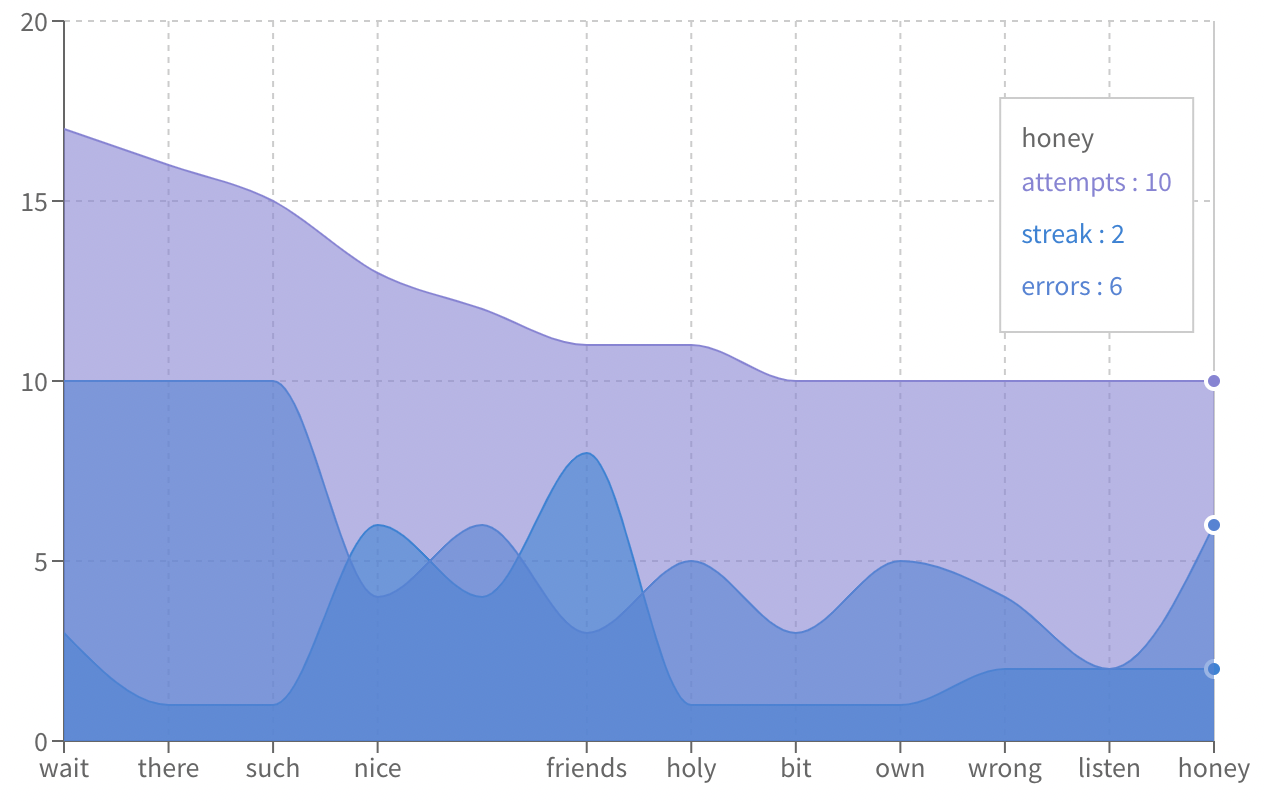
\includegraphics[width=1\textwidth]{assets/30.png}
       \end{minipage}
  \end{figure}
\end{frame}
The database provides information about the words, allowing the user to analyze the user's behavior and the words that the user is learning. The database has information about the words, the attempts, and the movies, as demonstrated in the figure-\ref{fig:database_data}. 
It's possible to see the words with the most errors, as demonstrated in the figure-\ref{fig:database_errors} (which containes the 12 words with the most errors in the database). The server will priorize those words to appear on the user screen, and the user will see the word more often. 
\begin{figure}[!h]
  \centering
  \caption{
  Streaks, erros and attempts of the users
  }
  \label{fig:database_users}
  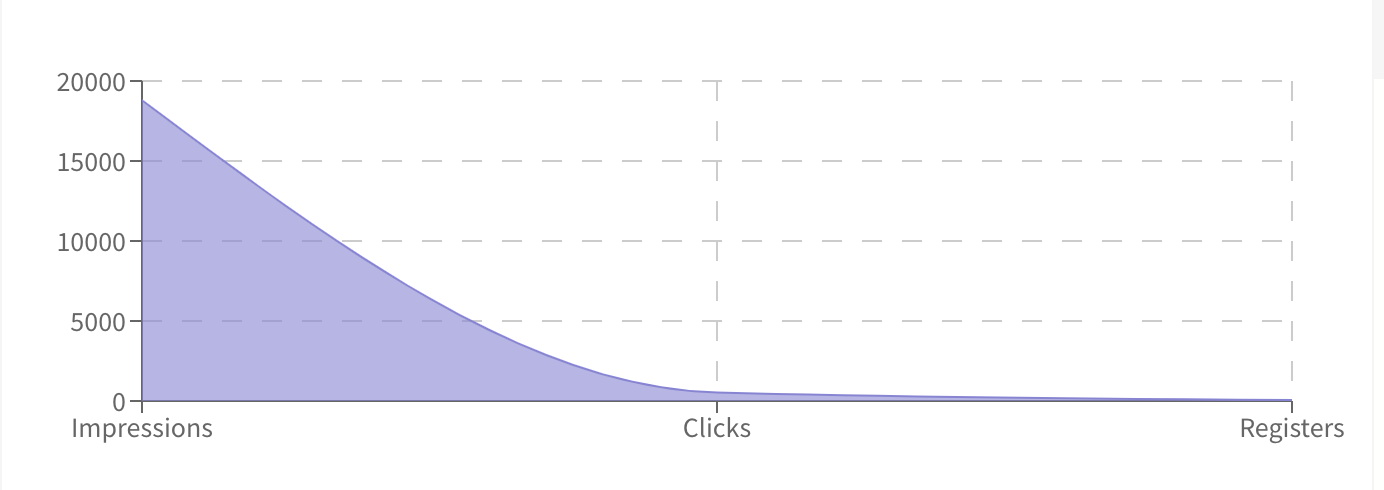
\includegraphics[width=0.50\textwidth]{assets/31.png}
\end{figure}
The server also knows the streaks, errors, and attempts of the users, as demonstrated in the figure-\ref{fig:database_users}. Some users already have tried to learn words 880 times. And is possible analise that 
most errors and appears of the word, more the users will train that word and more attempts will have, as possible see in the figure-\ref{fig:database_users}. \\
Until now the application has been well received by users, the database has been growing, and the application has been used by a significant number of users, 58 at the time of writing (16/06/2024). The tax of conversion follows that funnel of conversion, as demonstrated in the figure-\ref{fig:database_errors}. 
But is also possible see that the streaks (times that user saw the word without making a mistake) is growing, and the users are learning the words, as demonstrated in the figure-\ref{fig:database_users}. \\
When the streak line is bigger than the error line, the user is learning the word, and the server will decrease the priority of that word to appear on the user screen. \\
During that period the users have tried to learn the words of 22 movies and a total of 1049 words. It means that each movie tries to learn as a media of 47 words. with a media of 5.58 attempts per word with more than 1 error. And a medium of 2.98 errors per words with more than 1. \\


\section{
Conclusion
}
This work has successfully developed a browser extension, a website, and an app that aims to facilitate language learning by extracting subtitles from movie streaming sites. The extension utilizes Spaced Repetition System (SRS) techniques to gamify language learning, while the website provides statistics on user progress and supports multiple languages. The app allows users to study on any device. \\
Moving forward, several steps are planned for each application component. The extension will be expanded to other streaming sites, languages, and platforms and it will be integrated with other language-learning tools. The website will include interactive exercises, games, and customized learning experiences. The app will capture device information and improve communication with the website. \\
In addition, the application's backend will be enhanced with improvements to API routers and to the language manager. Web sockets will improve communication between the extension and the website. \\
Overall, this work demonstrates the potential of using technology to make language learning more engaging and accessible. By integrating language learning with everyday activities like watching movies, users can enhance their language skills in a fun and interactive way.\\







\bibliographystyle{sbc}
\bibliography{sbc-template}
\hfill \\
\hfill \\
\hfill \\
\hfill \\
\hfill \\
\hfill \\
\hfill \\
\hfill 
\centering

\begin{tabular}{@{}p{.5in}p{4in}@{}}
& \hrulefill \\
& \centerline{Guilherme A. Avelino} \\
\\ \\ \\ \\ 
\end{tabular}

\centering
\begin{tabular}{@{}p{.5in}p{4in}@{}}
& \hrulefill \\
& \centerline{J. Emanuel Cascone R. S.} \\
\\ \\
\end{tabular}

\end{document}